% POLYDIM_DEST
% destino: polydim/docs/
% nombre:  polydim_figures.tex
% autor:   ai.mpat.agt@gmail.com
% fecha:   2026-06-27
% uso:     % POLYDIM_DEST
% destino: polydim/docs/
% nombre:  polydim_figures.tex
% autor:   ai.mpat.agt@gmail.com
% fecha:   2026-06-27
% uso:     % POLYDIM_DEST
% destino: polydim/docs/
% nombre:  polydim_figures.tex
% autor:   ai.mpat.agt@gmail.com
% fecha:   2026-06-27
% uso:     % POLYDIM_DEST
% destino: polydim/docs/
% nombre:  polydim_figures.tex
% autor:   ai.mpat.agt@gmail.com
% fecha:   2026-06-27
% uso:     \input{polydim_figures} en polydim_paper_arxiv.tex
%          O compilar standalone con pdflatex para preview
%
% Figuras incluidas:
%   Fig 1: PROJECT como funtor (G → E_X)
%   Fig 2: Arquitectura dos capas (Algebraic / Implementation)
%   Fig 3: Protocolo ALIGN AI↔AI
%   Fig 4: Sistema de tipos dimensional (el mismo objeto, 4 proyecciones)

\documentclass[tikz,border=6pt]{standalone}
\usepackage{tikz}
\usepackage{amsmath,amssymb}
\usepackage{xcolor}
\usetikzlibrary{
  arrows.meta,
  positioning,
  shapes.geometric,
  shapes.misc,
  fit,
  backgrounds,
  decorations.pathreplacing,
  matrix,
  calc,
  shadows.blur
}

%% ============================================================
%% Color palette
%% ============================================================
\definecolor{polyblue}{RGB}{30,80,160}
\definecolor{polylightblue}{RGB}{200,220,255}
\definecolor{polygreen}{RGB}{20,140,60}
\definecolor{polylightgreen}{RGB}{200,245,215}
\definecolor{polyorange}{RGB}{200,100,20}
\definecolor{polylightorange}{RGB}{255,230,200}
\definecolor{polyred}{RGB}{180,30,30}
\definecolor{polylightred}{RGB}{255,210,210}
\definecolor{polygray}{RGB}{90,90,90}
\definecolor{polylightgray}{RGB}{240,240,240}
\definecolor{polypurple}{RGB}{120,30,180}
\definecolor{polylightpurple}{RGB}{230,200,255}

%% ============================================================
%% Common TikZ styles
%% ============================================================
\tikzset{
  %% Category box
  catbox/.style={
    draw=#1, fill=#1!10, rounded corners=6pt,
    minimum width=3.2cm, minimum height=2.4cm,
    line width=1.2pt, font=\small
  },
  %% Object node
  objnode/.style={
    draw=#1, fill=#1!20, circle,
    minimum size=0.55cm, line width=0.8pt,
    font=\scriptsize\bfseries, text=#1!60!black
  },
  %% Morphism arrow
  morpharrow/.style={
    -{Latex[length=4pt,width=3pt]},
    draw=#1, line width=0.9pt
  },
  %% Functor arrow
  functarrow/.style={
    -{Latex[length=6pt,width=5pt]},
    draw=polyorange, line width=1.8pt,
    double=polylightorange, double distance=1.5pt
  },
  %% Layer box
  layerbox/.style={
    draw=#1, fill=#1!8, rounded corners=4pt,
    minimum width=8cm, line width=1.2pt,
    font=\small\bfseries, text=#1
  },
  %% Primitive node
  primnode/.style={
    draw=#1, fill=#1!15, rounded corners=3pt,
    minimum width=2.6cm, minimum height=0.65cm,
    line width=0.8pt, font=\small
  },
}

\begin{document}

%% ============================================================
%% FIGURE 1: PROJECT as a Functor  G → E_X
%% ============================================================
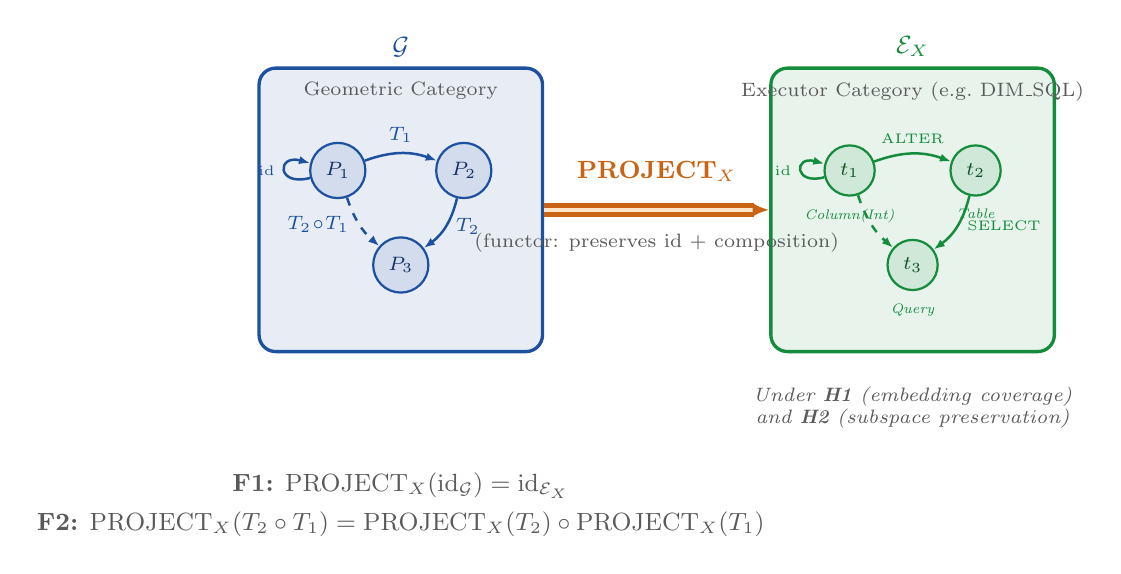
\begin{tikzpicture}[node distance=1cm and 3.8cm]

  %% ── Geometric category G ─────────────────────────────────
  \node[catbox=polyblue, minimum width=3.6cm, minimum height=3.6cm]
    (Gbox) at (0,0) {};
  \node[above=0pt of Gbox.north, font=\small\bfseries\color{polyblue}]
    {$\mathcal{G}$};
  \node[below=2pt of Gbox.north, font=\scriptsize\color{polygray}]
    {Geometric Category};

  % Objects in G
  \node[objnode=polyblue] (P1) at (-0.8, 0.5) {$P_1$};
  \node[objnode=polyblue] (P2) at ( 0.8, 0.5) {$P_2$};
  \node[objnode=polyblue] (P3) at ( 0.0,-0.7) {$P_3$};

  % Morphisms in G (transformations T)
  \draw[morpharrow=polyblue]
    (P1) to[bend left=20]
    node[above, font=\scriptsize, text=polyblue] {$T_1$} (P2);
  \draw[morpharrow=polyblue]
    (P2) to[bend left=20]
    node[right, font=\scriptsize, text=polyblue] {$T_2$} (P3);
  \draw[morpharrow=polyblue, dashed]
    (P1) to[bend right=15]
    node[left, font=\scriptsize, text=polyblue] {$T_2\!\circ\!T_1$} (P3);

  % Identity
  \draw[morpharrow=polyblue]
    (P1) to[loop left, looseness=6]
    node[left, font=\tiny, text=polyblue] {$\mathrm{id}$} (P1);

  %% ── Executor category E_X ────────────────────────────────
  \node[catbox=polygreen, minimum width=3.6cm, minimum height=3.6cm]
    (Ebox) at (6.5, 0) {};
  \node[above=0pt of Ebox.north, font=\small\bfseries\color{polygreen}]
    {$\mathcal{E}_X$};
  \node[below=2pt of Ebox.north, font=\scriptsize\color{polygray}]
    {Executor Category (e.g.\ DIM\_SQL)};

  % Objects in E_X (types)
  \node[objnode=polygreen] (t1) at (5.7, 0.5)
    {\scriptsize $t_1$};
  \node[objnode=polygreen] (t2) at (7.3, 0.5)
    {\scriptsize $t_2$};
  \node[objnode=polygreen] (t3) at (6.5,-0.7)
    {\scriptsize $t_3$};

  % Type labels
  \node[below=1pt of t1, font=\tiny\itshape, text=polygreen]
    {Column(Int)};
  \node[below=1pt of t2, font=\tiny\itshape, text=polygreen]
    {Table};
  \node[below=1pt of t3, font=\tiny\itshape, text=polygreen]
    {Query};

  % Morphisms in E_X (type maps)
  \draw[morpharrow=polygreen]
    (t1) to[bend left=20]
    node[above, font=\tiny, text=polygreen] {ALTER} (t2);
  \draw[morpharrow=polygreen]
    (t2) to[bend left=20]
    node[right, font=\tiny, text=polygreen] {SELECT} (t3);
  \draw[morpharrow=polygreen, dashed]
    (t1) to[bend right=15]
    node[left, font=\tiny, text=polygreen] {} (t3);

  \draw[morpharrow=polygreen]
    (t1) to[loop left, looseness=6]
    node[left, font=\tiny, text=polygreen] {$\mathrm{id}$} (t1);

  %% ── PROJECT_X functor arrow ───────────────────────────────
  \draw[functarrow]
    ($(Gbox.east)+(0,0)$) -- node[above=6pt, font=\small\bfseries\color{polyorange}]
    {$\mathbf{PROJECT}_X$}
    node[below=4pt, font=\scriptsize\color{polygray}]
    {(functor: preserves id + composition)}
    ($(Ebox.west)+(0,0)$);

  %% ── Functor equations ────────────────────────────────────
  \node[below=1.4cm of Gbox.south, anchor=north,
        font=\small, text=polygray, align=center] {
    \textbf{F1:} $\mathrm{PROJECT}_X(\mathrm{id}_\mathcal{G}) = \mathrm{id}_{\mathcal{E}_X}$ \\[3pt]
    \textbf{F2:} $\mathrm{PROJECT}_X(T_2 \circ T_1) =
                  \mathrm{PROJECT}_X(T_2) \circ \mathrm{PROJECT}_X(T_1)$
  };

  %% ── H2 annotation ────────────────────────────────────────
  \node[below=0.3cm of Ebox.south, anchor=north,
        font=\scriptsize\itshape, text=polygray, align=center] {
    Under \textbf{H1} (embedding coverage) \\
    and \textbf{H2} (subspace preservation)
  };

\end{tikzpicture}

\bigskip
%% ============================================================
%% FIGURE 2: Two-Layer Architecture
%% ============================================================
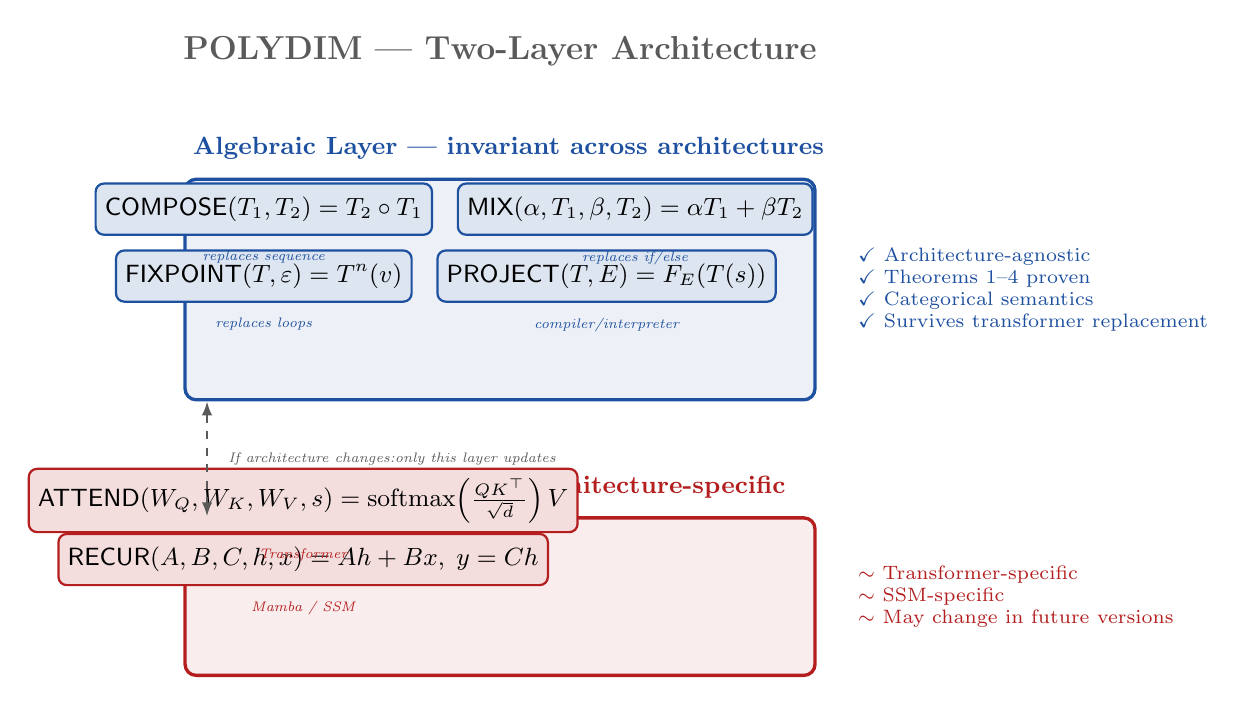
\begin{tikzpicture}[node distance=0.5cm]

  %% Title
  \node[font=\large\bfseries, text=polygray] (title) at (4, 0)
    {POLYDIM — Two-Layer Architecture};

  %% ── ALGEBRAIC LAYER ──────────────────────────────────────
  \node[layerbox=polyblue, minimum height=2.8cm,
        below=0.8cm of title, anchor=north] (alglayer) at (4, -0.8) {};

  \node[above=3pt of alglayer.north west, anchor=south west,
        font=\small\bfseries, text=polyblue]
    {Algebraic Layer — invariant across architectures};

  % Primitives
  \node[primnode=polyblue] (compose) at (1.0,-2.0)
    {$\mathsf{COMPOSE}(T_1, T_2) = T_2 \circ T_1$};
  \node[primnode=polyblue, right=0.3cm of compose] (mix)
    {$\mathsf{MIX}(\alpha, T_1, \beta, T_2) = \alpha T_1 + \beta T_2$};
  \node[primnode=polyblue] (fix) at (1.0,-2.85)
    {$\mathsf{FIXPOINT}(T, \varepsilon) = T^n(v)$};
  \node[primnode=polyblue, right=0.3cm of fix] (proj)
    {$\mathsf{PROJECT}(T, E) = F_E(T(s))$};

  % Property tags
  \node[below=2pt of compose.south, font=\tiny\itshape, text=polyblue]
    {replaces sequence};
  \node[below=2pt of mix.south, font=\tiny\itshape, text=polyblue]
    {replaces if/else};
  \node[below=2pt of fix.south, font=\tiny\itshape, text=polyblue]
    {replaces loops};
  \node[below=2pt of proj.south, font=\tiny\itshape, text=polyblue]
    {compiler/interpreter};

  %% ── IMPLEMENTATION LAYER ─────────────────────────────────
  \node[layerbox=polyred, minimum height=2.0cm,
        below=1.1cm of alglayer.south, anchor=north] (impllayer) at (4,-4.8) {};

  \node[above=3pt of impllayer.north west, anchor=south west,
        font=\small\bfseries, text=polyred]
    {Implementation Layer — architecture-specific};

  \node[primnode=polyred] (attend) at (1.5,-5.7)
    {$\mathsf{ATTEND}(W_Q, W_K, W_V, s) = \mathrm{softmax}\!\left(\tfrac{QK^\top}{\sqrt{d}}\right)V$};
  \node[primnode=polyred] (recur) at (1.5,-6.45)
    {$\mathsf{RECUR}(A, B, C, h, x) = Ah + Bx,\; y = Ch$};

  \node[below=2pt of attend.south, font=\tiny\itshape, text=polyred]
    {Transformer};
  \node[below=2pt of recur.south, font=\tiny\itshape, text=polyred]
    {Mamba / SSM};

  %% ── Separator arrow ──────────────────────────────────────
  \draw[{Latex[length=5pt]}-{Latex[length=5pt]},
        draw=polygray, dashed, line width=0.7pt]
    ($(alglayer.south west)+(0.3,0)$) --
    node[right=4pt, font=\tiny\itshape, text=polygray]
      {If architecture changes:\\
       only this layer updates}
    ($(impllayer.north west)+(0.3,0)$);

  %% ── Property annotations ─────────────────────────────────
  \node[right=0.4cm of alglayer.east, anchor=west,
        font=\scriptsize, text=polyblue, align=left] {
    \checkmark\ Architecture-agnostic \\
    \checkmark\ Theorems 1--4 proven \\
    \checkmark\ Categorical semantics \\
    \checkmark\ Survives transformer replacement
  };

  \node[right=0.4cm of impllayer.east, anchor=west,
        font=\scriptsize, text=polyred, align=left] {
    $\sim$\ Transformer-specific \\
    $\sim$\ SSM-specific \\
    $\sim$\ May change in future versions
  };

\end{tikzpicture}

\bigskip
%% ============================================================
%% FIGURE 3: ALIGN Protocol — AI-to-AI Communication
%% ============================================================
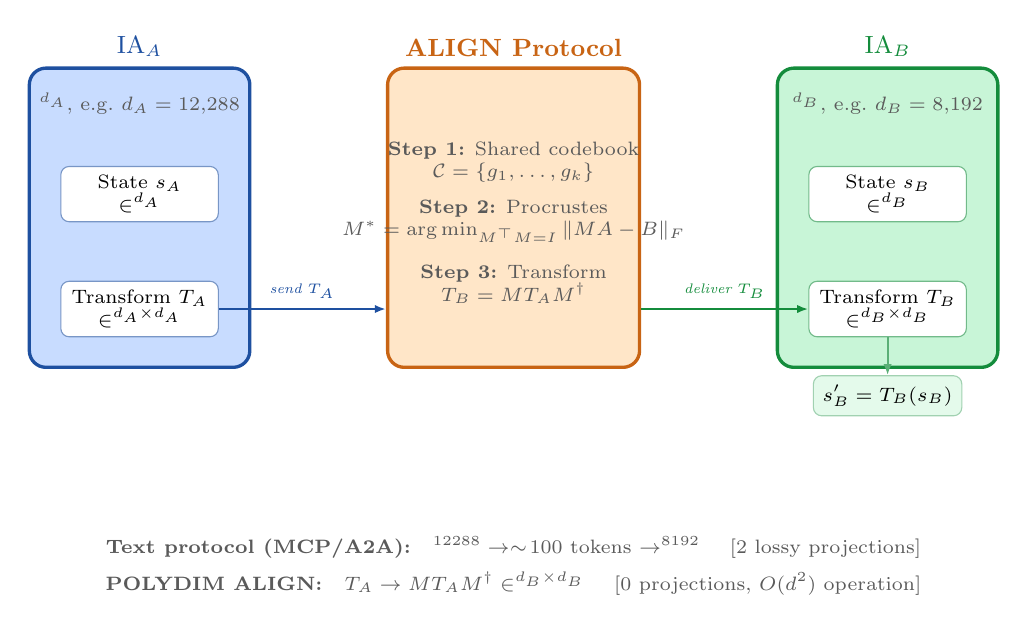
\begin{tikzpicture}[node distance=1.2cm and 2.5cm]

  %% IA_A box
  \node[draw=polyblue, fill=polylightblue, rounded corners=6pt,
        minimum width=2.8cm, minimum height=3.8cm, line width=1.2pt]
    (IA_A) at (0, 0) {};
  \node[above=0pt of IA_A.north, font=\small\bfseries\color{polyblue}]
    {$\mathrm{IA}_A$};
  \node[below=6pt of IA_A.north, font=\scriptsize\color{polygray}]
    {$\RR^{d_A}$, e.g.\ $d_A = 12{,}288$};

  \node[draw=polyblue!60, fill=white, rounded corners=3pt,
        minimum width=2.0cm, font=\scriptsize, align=center]
    (stateA) at (0, 0.3) {State $s_A$\\$\in \RR^{d_A}$};
  \node[draw=polyblue!60, fill=white, rounded corners=3pt,
        minimum width=2.0cm, font=\scriptsize, align=center,
        below=0.2cm of stateA]
    (transA) at (0,-0.6) {Transform $T_A$\\$\in \RR^{d_A \times d_A}$};

  %% IA_B box
  \node[draw=polygreen, fill=polylightgreen, rounded corners=6pt,
        minimum width=2.8cm, minimum height=3.8cm, line width=1.2pt]
    (IA_B) at (9.5, 0) {};
  \node[above=0pt of IA_B.north, font=\small\bfseries\color{polygreen}]
    {$\mathrm{IA}_B$};
  \node[below=6pt of IA_B.north, font=\scriptsize\color{polygray}]
    {$\RR^{d_B}$, e.g.\ $d_B = 8{,}192$};

  \node[draw=polygreen!60, fill=white, rounded corners=3pt,
        minimum width=2.0cm, font=\scriptsize, align=center]
    (stateB) at (9.5, 0.3) {State $s_B$\\$\in \RR^{d_B}$};
  \node[draw=polygreen!60, fill=white, rounded corners=3pt,
        minimum width=2.0cm, font=\scriptsize, align=center,
        below=0.2cm of stateB]
    (transB) at (9.5,-0.6) {Transform $T_B$\\$\in \RR^{d_B \times d_B}$};

  %% ALIGN box in the middle
  \node[draw=polyorange, fill=polylightorange, rounded corners=6pt,
        minimum width=3.2cm, minimum height=3.8cm, line width=1.2pt]
    (align) at (4.75, 0) {};
  \node[above=0pt of align.north, font=\small\bfseries\color{polyorange}]
    {ALIGN Protocol};

  \node[font=\scriptsize, align=center, text=polygray]
    at (4.75, 0.7) {
      \textbf{Step 1:} Shared codebook \\
      $\mathcal{C} = \{g_1, \ldots, g_k\}$
    };
  \node[font=\scriptsize, align=center, text=polygray]
    at (4.75, -0.05) {
      \textbf{Step 2:} Procrustes \\
      $M^* = \arg\min_{M^\top M=I} \|MA-B\|_F$
    };
  \node[font=\scriptsize, align=center, text=polygray]
    at (4.75, -0.85) {
      \textbf{Step 3:} Transform \\
      $T_B = M T_A M^\dagger$
    };

  %% Arrows
  \draw[-{Latex[length=4pt]}, polyblue, line width=0.9pt]
    (transA.east) -- node[above, font=\tiny\itshape] {send $T_A$}
    (align.west |- transA.east);

  \draw[-{Latex[length=4pt]}, polygreen, line width=0.9pt]
    (align.east |- transB.west) --
    node[above, font=\tiny\itshape] {deliver $T_B$}
    (transB.west);

  %% Application
  \node[draw=polygreen!40, fill=polylightgreen!50, rounded corners=3pt,
        font=\scriptsize, align=center, below=0.5cm of stateB]
    (apply) at (9.5,-1.5) {$s_B' = T_B(s_B)$};
  \draw[-{Latex[length=4pt]}, polygreen!70, line width=0.7pt]
    (transB.south) -- (apply.north);

  %% Comparison
  \node[below=2.0cm of align.south, anchor=north,
        font=\scriptsize, align=center, text=polygray] {
    \textbf{Text protocol (MCP/A2A):}\quad
    $\RR^{12288} \to \sim\!100$ tokens $\to \RR^{8192}$
    \quad [2 lossy projections] \\[4pt]
    \textbf{POLYDIM ALIGN:}\quad
    $T_A \to M T_A M^\dagger \in \RR^{d_B \times d_B}$
    \quad [0 projections, $O(d^2)$ operation]
  };

\end{tikzpicture}

\bigskip
%% ============================================================
%% FIGURE 4: Dimensional Type System
%% ============================================================
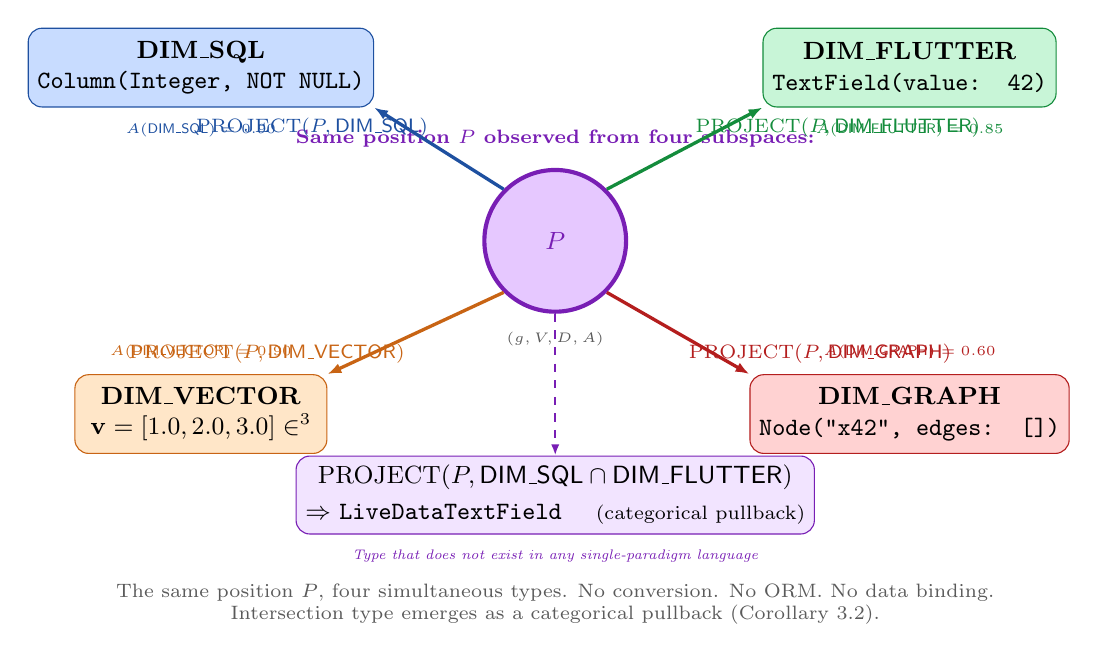
\begin{tikzpicture}[node distance=0.8cm and 1.5cm]

  %% Central position P
  \node[draw=polypurple, fill=polylightpurple, circle,
        minimum size=1.8cm, line width=1.5pt,
        font=\small\bfseries, text=polypurple]
    (P) at (0, 0) {$P$};

  \node[below=3pt of P, font=\tiny\color{polygray}]
    {$(g, V, D, A)$};

  \node[above=4pt of P.north, font=\scriptsize\bfseries, text=polypurple]
    {Same position $P$ observed from four subspaces:};

  %% DIM_SQL projection
  \node[draw=polyblue, fill=polylightblue, rounded corners=5pt,
        minimum width=3.2cm, minimum height=1.0cm,
        font=\small, align=center]
    (sql) at (-4.5, 2.2) {
      \textbf{DIM\_SQL} \\
      \small\texttt{Column(Integer, NOT NULL)}
    };
  \draw[-{Latex[length=5pt]}, polyblue, line width=1.2pt]
    (P.north west) -- node[above left, font=\scriptsize, text=polyblue]
    {$\mathrm{PROJECT}(P, \mathsf{DIM\_SQL})$} (sql.south east);
  \node[below=2pt of sql.south, font=\tiny\itshape, text=polyblue]
    {$A(\mathsf{DIM\_SQL}) = 0.90$};

  %% DIM_FLUTTER projection
  \node[draw=polygreen, fill=polylightgreen, rounded corners=5pt,
        minimum width=3.2cm, minimum height=1.0cm,
        font=\small, align=center]
    (flutter) at (4.5, 2.2) {
      \textbf{DIM\_FLUTTER} \\
      \small\texttt{TextField(value: 42)}
    };
  \draw[-{Latex[length=5pt]}, polygreen, line width=1.2pt]
    (P.north east) -- node[above right, font=\scriptsize, text=polygreen]
    {$\mathrm{PROJECT}(P, \mathsf{DIM\_FLUTTER})$} (flutter.south west);
  \node[below=2pt of flutter.south, font=\tiny\itshape, text=polygreen]
    {$A(\mathsf{DIM\_FLUTTER}) = 0.85$};

  %% DIM_VECTOR projection
  \node[draw=polyorange, fill=polylightorange, rounded corners=5pt,
        minimum width=3.2cm, minimum height=1.0cm,
        font=\small, align=center]
    (vector) at (-4.5, -2.2) {
      \textbf{DIM\_VECTOR} \\
      \small$\mathbf{v} = [1.0, 2.0, 3.0] \in \RR^3$
    };
  \draw[-{Latex[length=5pt]}, polyorange, line width=1.2pt]
    (P.south west) -- node[below left, font=\scriptsize, text=polyorange]
    {$\mathrm{PROJECT}(P, \mathsf{DIM\_VECTOR})$} (vector.north east);
  \node[above=2pt of vector.north, font=\tiny\itshape, text=polyorange]
    {$A(\mathsf{DIM\_VECTOR}) = 0.90$};

  %% DIM_GRAPH projection
  \node[draw=polyred, fill=polylightred, rounded corners=5pt,
        minimum width=3.2cm, minimum height=1.0cm,
        font=\small, align=center]
    (graph) at (4.5, -2.2) {
      \textbf{DIM\_GRAPH} \\
      \small\texttt{Node("x42", edges: [])}
    };
  \draw[-{Latex[length=5pt]}, polyred, line width=1.2pt]
    (P.south east) -- node[below right, font=\scriptsize, text=polyred]
    {$\mathrm{PROJECT}(P, \mathsf{DIM\_GRAPH})$} (graph.north west);
  \node[above=2pt of graph.north, font=\tiny\itshape, text=polyred]
    {$A(\mathsf{DIM\_GRAPH}) = 0.60$};

  %% Intersection type (pullback)
  \node[draw=polypurple, fill=polylightpurple!50, rounded corners=5pt,
        minimum width=4.0cm, minimum height=0.9cm,
        font=\small, align=center, below=1.8cm of P]
    (intersect) {
      $\mathrm{PROJECT}(P, \mathsf{DIM\_SQL} \cap \mathsf{DIM\_FLUTTER})$ \\[2pt]
      \small $\Rightarrow$ \texttt{LiveDataTextField} \quad
      \scriptsize(categorical pullback)
    };
  \draw[-{Latex[length=4pt]}, polypurple, dashed, line width=0.9pt]
    (P.south) -- (intersect.north);
  \node[below=2pt of intersect.south, font=\tiny\itshape, text=polypurple]
    {Type that does not exist in any single-paradigm language};

  %% Caption
  \node[below=0.5cm of intersect.south, anchor=north,
        font=\scriptsize, text=polygray, align=center] {
    The same position $P$, four simultaneous types. No conversion. No ORM. No data binding. \\
    Intersection type emerges as a categorical pullback (Corollary~3.2).
  };

\end{tikzpicture}

\end{document}
 en polydim_paper_arxiv.tex
%          O compilar standalone con pdflatex para preview
%
% Figuras incluidas:
%   Fig 1: PROJECT como funtor (G → E_X)
%   Fig 2: Arquitectura dos capas (Algebraic / Implementation)
%   Fig 3: Protocolo ALIGN AI↔AI
%   Fig 4: Sistema de tipos dimensional (el mismo objeto, 4 proyecciones)

\documentclass[tikz,border=6pt]{standalone}
\usepackage{tikz}
\usepackage{amsmath,amssymb}
\usepackage{xcolor}
\usetikzlibrary{
  arrows.meta,
  positioning,
  shapes.geometric,
  shapes.misc,
  fit,
  backgrounds,
  decorations.pathreplacing,
  matrix,
  calc,
  shadows.blur
}

%% ============================================================
%% Color palette
%% ============================================================
\definecolor{polyblue}{RGB}{30,80,160}
\definecolor{polylightblue}{RGB}{200,220,255}
\definecolor{polygreen}{RGB}{20,140,60}
\definecolor{polylightgreen}{RGB}{200,245,215}
\definecolor{polyorange}{RGB}{200,100,20}
\definecolor{polylightorange}{RGB}{255,230,200}
\definecolor{polyred}{RGB}{180,30,30}
\definecolor{polylightred}{RGB}{255,210,210}
\definecolor{polygray}{RGB}{90,90,90}
\definecolor{polylightgray}{RGB}{240,240,240}
\definecolor{polypurple}{RGB}{120,30,180}
\definecolor{polylightpurple}{RGB}{230,200,255}

%% ============================================================
%% Common TikZ styles
%% ============================================================
\tikzset{
  %% Category box
  catbox/.style={
    draw=#1, fill=#1!10, rounded corners=6pt,
    minimum width=3.2cm, minimum height=2.4cm,
    line width=1.2pt, font=\small
  },
  %% Object node
  objnode/.style={
    draw=#1, fill=#1!20, circle,
    minimum size=0.55cm, line width=0.8pt,
    font=\scriptsize\bfseries, text=#1!60!black
  },
  %% Morphism arrow
  morpharrow/.style={
    -{Latex[length=4pt,width=3pt]},
    draw=#1, line width=0.9pt
  },
  %% Functor arrow
  functarrow/.style={
    -{Latex[length=6pt,width=5pt]},
    draw=polyorange, line width=1.8pt,
    double=polylightorange, double distance=1.5pt
  },
  %% Layer box
  layerbox/.style={
    draw=#1, fill=#1!8, rounded corners=4pt,
    minimum width=8cm, line width=1.2pt,
    font=\small\bfseries, text=#1
  },
  %% Primitive node
  primnode/.style={
    draw=#1, fill=#1!15, rounded corners=3pt,
    minimum width=2.6cm, minimum height=0.65cm,
    line width=0.8pt, font=\small
  },
}

\begin{document}

%% ============================================================
%% FIGURE 1: PROJECT as a Functor  G → E_X
%% ============================================================
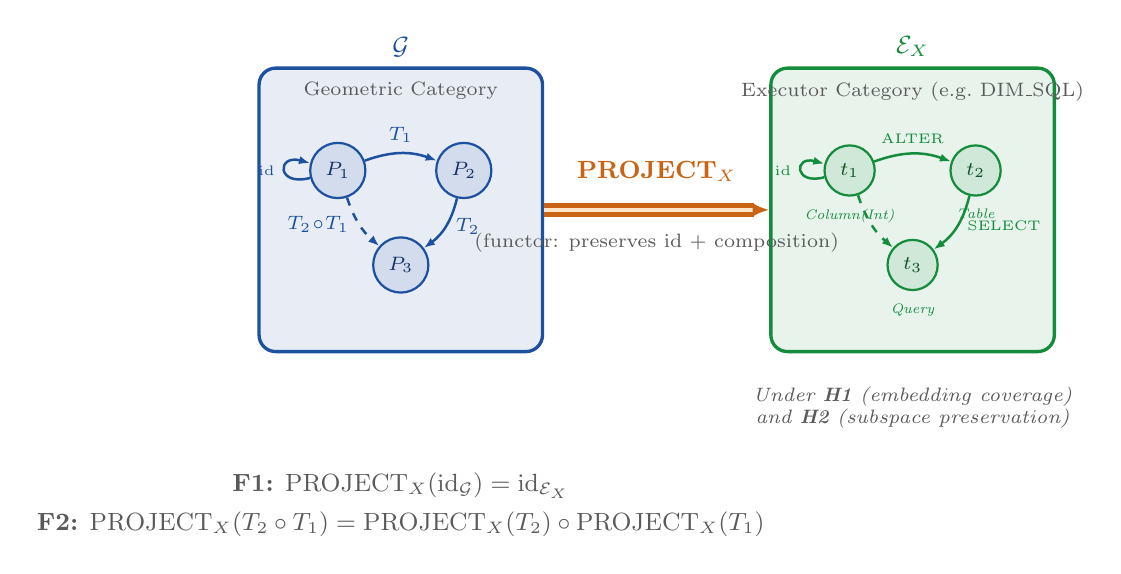
\begin{tikzpicture}[node distance=1cm and 3.8cm]

  %% ── Geometric category G ─────────────────────────────────
  \node[catbox=polyblue, minimum width=3.6cm, minimum height=3.6cm]
    (Gbox) at (0,0) {};
  \node[above=0pt of Gbox.north, font=\small\bfseries\color{polyblue}]
    {$\mathcal{G}$};
  \node[below=2pt of Gbox.north, font=\scriptsize\color{polygray}]
    {Geometric Category};

  % Objects in G
  \node[objnode=polyblue] (P1) at (-0.8, 0.5) {$P_1$};
  \node[objnode=polyblue] (P2) at ( 0.8, 0.5) {$P_2$};
  \node[objnode=polyblue] (P3) at ( 0.0,-0.7) {$P_3$};

  % Morphisms in G (transformations T)
  \draw[morpharrow=polyblue]
    (P1) to[bend left=20]
    node[above, font=\scriptsize, text=polyblue] {$T_1$} (P2);
  \draw[morpharrow=polyblue]
    (P2) to[bend left=20]
    node[right, font=\scriptsize, text=polyblue] {$T_2$} (P3);
  \draw[morpharrow=polyblue, dashed]
    (P1) to[bend right=15]
    node[left, font=\scriptsize, text=polyblue] {$T_2\!\circ\!T_1$} (P3);

  % Identity
  \draw[morpharrow=polyblue]
    (P1) to[loop left, looseness=6]
    node[left, font=\tiny, text=polyblue] {$\mathrm{id}$} (P1);

  %% ── Executor category E_X ────────────────────────────────
  \node[catbox=polygreen, minimum width=3.6cm, minimum height=3.6cm]
    (Ebox) at (6.5, 0) {};
  \node[above=0pt of Ebox.north, font=\small\bfseries\color{polygreen}]
    {$\mathcal{E}_X$};
  \node[below=2pt of Ebox.north, font=\scriptsize\color{polygray}]
    {Executor Category (e.g.\ DIM\_SQL)};

  % Objects in E_X (types)
  \node[objnode=polygreen] (t1) at (5.7, 0.5)
    {\scriptsize $t_1$};
  \node[objnode=polygreen] (t2) at (7.3, 0.5)
    {\scriptsize $t_2$};
  \node[objnode=polygreen] (t3) at (6.5,-0.7)
    {\scriptsize $t_3$};

  % Type labels
  \node[below=1pt of t1, font=\tiny\itshape, text=polygreen]
    {Column(Int)};
  \node[below=1pt of t2, font=\tiny\itshape, text=polygreen]
    {Table};
  \node[below=1pt of t3, font=\tiny\itshape, text=polygreen]
    {Query};

  % Morphisms in E_X (type maps)
  \draw[morpharrow=polygreen]
    (t1) to[bend left=20]
    node[above, font=\tiny, text=polygreen] {ALTER} (t2);
  \draw[morpharrow=polygreen]
    (t2) to[bend left=20]
    node[right, font=\tiny, text=polygreen] {SELECT} (t3);
  \draw[morpharrow=polygreen, dashed]
    (t1) to[bend right=15]
    node[left, font=\tiny, text=polygreen] {} (t3);

  \draw[morpharrow=polygreen]
    (t1) to[loop left, looseness=6]
    node[left, font=\tiny, text=polygreen] {$\mathrm{id}$} (t1);

  %% ── PROJECT_X functor arrow ───────────────────────────────
  \draw[functarrow]
    ($(Gbox.east)+(0,0)$) -- node[above=6pt, font=\small\bfseries\color{polyorange}]
    {$\mathbf{PROJECT}_X$}
    node[below=4pt, font=\scriptsize\color{polygray}]
    {(functor: preserves id + composition)}
    ($(Ebox.west)+(0,0)$);

  %% ── Functor equations ────────────────────────────────────
  \node[below=1.4cm of Gbox.south, anchor=north,
        font=\small, text=polygray, align=center] {
    \textbf{F1:} $\mathrm{PROJECT}_X(\mathrm{id}_\mathcal{G}) = \mathrm{id}_{\mathcal{E}_X}$ \\[3pt]
    \textbf{F2:} $\mathrm{PROJECT}_X(T_2 \circ T_1) =
                  \mathrm{PROJECT}_X(T_2) \circ \mathrm{PROJECT}_X(T_1)$
  };

  %% ── H2 annotation ────────────────────────────────────────
  \node[below=0.3cm of Ebox.south, anchor=north,
        font=\scriptsize\itshape, text=polygray, align=center] {
    Under \textbf{H1} (embedding coverage) \\
    and \textbf{H2} (subspace preservation)
  };

\end{tikzpicture}

\bigskip
%% ============================================================
%% FIGURE 2: Two-Layer Architecture
%% ============================================================
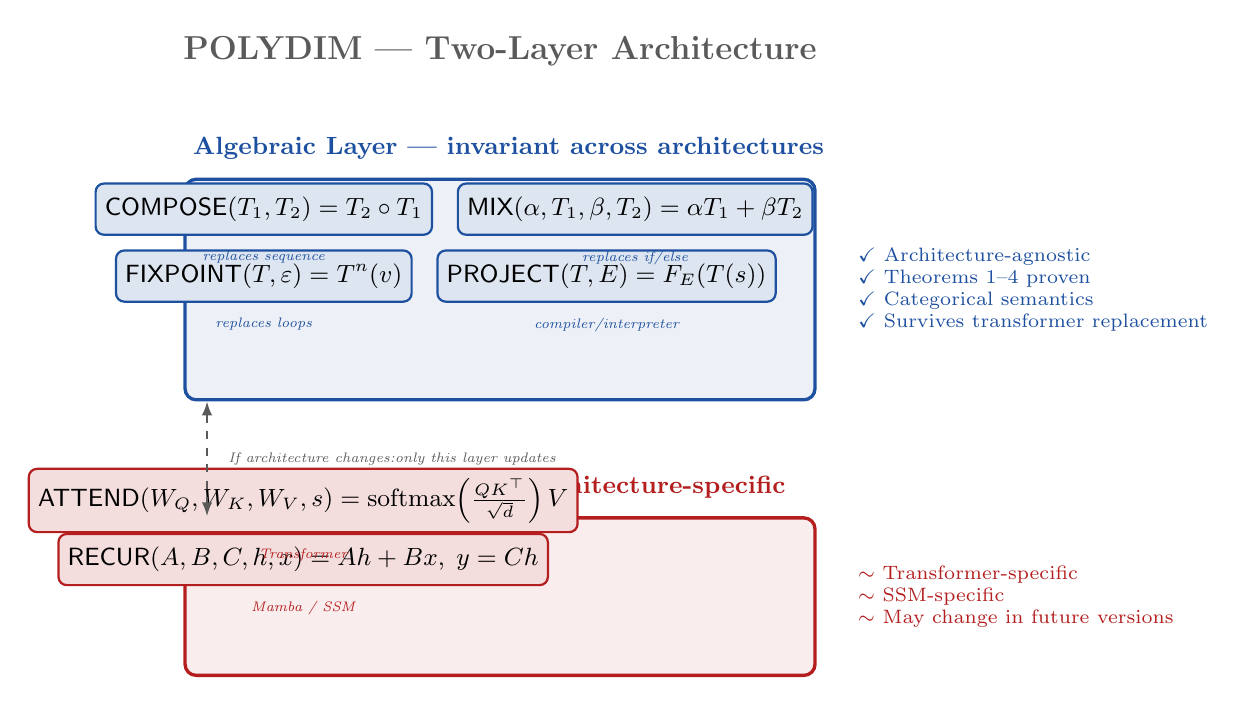
\begin{tikzpicture}[node distance=0.5cm]

  %% Title
  \node[font=\large\bfseries, text=polygray] (title) at (4, 0)
    {POLYDIM — Two-Layer Architecture};

  %% ── ALGEBRAIC LAYER ──────────────────────────────────────
  \node[layerbox=polyblue, minimum height=2.8cm,
        below=0.8cm of title, anchor=north] (alglayer) at (4, -0.8) {};

  \node[above=3pt of alglayer.north west, anchor=south west,
        font=\small\bfseries, text=polyblue]
    {Algebraic Layer — invariant across architectures};

  % Primitives
  \node[primnode=polyblue] (compose) at (1.0,-2.0)
    {$\mathsf{COMPOSE}(T_1, T_2) = T_2 \circ T_1$};
  \node[primnode=polyblue, right=0.3cm of compose] (mix)
    {$\mathsf{MIX}(\alpha, T_1, \beta, T_2) = \alpha T_1 + \beta T_2$};
  \node[primnode=polyblue] (fix) at (1.0,-2.85)
    {$\mathsf{FIXPOINT}(T, \varepsilon) = T^n(v)$};
  \node[primnode=polyblue, right=0.3cm of fix] (proj)
    {$\mathsf{PROJECT}(T, E) = F_E(T(s))$};

  % Property tags
  \node[below=2pt of compose.south, font=\tiny\itshape, text=polyblue]
    {replaces sequence};
  \node[below=2pt of mix.south, font=\tiny\itshape, text=polyblue]
    {replaces if/else};
  \node[below=2pt of fix.south, font=\tiny\itshape, text=polyblue]
    {replaces loops};
  \node[below=2pt of proj.south, font=\tiny\itshape, text=polyblue]
    {compiler/interpreter};

  %% ── IMPLEMENTATION LAYER ─────────────────────────────────
  \node[layerbox=polyred, minimum height=2.0cm,
        below=1.1cm of alglayer.south, anchor=north] (impllayer) at (4,-4.8) {};

  \node[above=3pt of impllayer.north west, anchor=south west,
        font=\small\bfseries, text=polyred]
    {Implementation Layer — architecture-specific};

  \node[primnode=polyred] (attend) at (1.5,-5.7)
    {$\mathsf{ATTEND}(W_Q, W_K, W_V, s) = \mathrm{softmax}\!\left(\tfrac{QK^\top}{\sqrt{d}}\right)V$};
  \node[primnode=polyred] (recur) at (1.5,-6.45)
    {$\mathsf{RECUR}(A, B, C, h, x) = Ah + Bx,\; y = Ch$};

  \node[below=2pt of attend.south, font=\tiny\itshape, text=polyred]
    {Transformer};
  \node[below=2pt of recur.south, font=\tiny\itshape, text=polyred]
    {Mamba / SSM};

  %% ── Separator arrow ──────────────────────────────────────
  \draw[{Latex[length=5pt]}-{Latex[length=5pt]},
        draw=polygray, dashed, line width=0.7pt]
    ($(alglayer.south west)+(0.3,0)$) --
    node[right=4pt, font=\tiny\itshape, text=polygray]
      {If architecture changes:\\
       only this layer updates}
    ($(impllayer.north west)+(0.3,0)$);

  %% ── Property annotations ─────────────────────────────────
  \node[right=0.4cm of alglayer.east, anchor=west,
        font=\scriptsize, text=polyblue, align=left] {
    \checkmark\ Architecture-agnostic \\
    \checkmark\ Theorems 1--4 proven \\
    \checkmark\ Categorical semantics \\
    \checkmark\ Survives transformer replacement
  };

  \node[right=0.4cm of impllayer.east, anchor=west,
        font=\scriptsize, text=polyred, align=left] {
    $\sim$\ Transformer-specific \\
    $\sim$\ SSM-specific \\
    $\sim$\ May change in future versions
  };

\end{tikzpicture}

\bigskip
%% ============================================================
%% FIGURE 3: ALIGN Protocol — AI-to-AI Communication
%% ============================================================
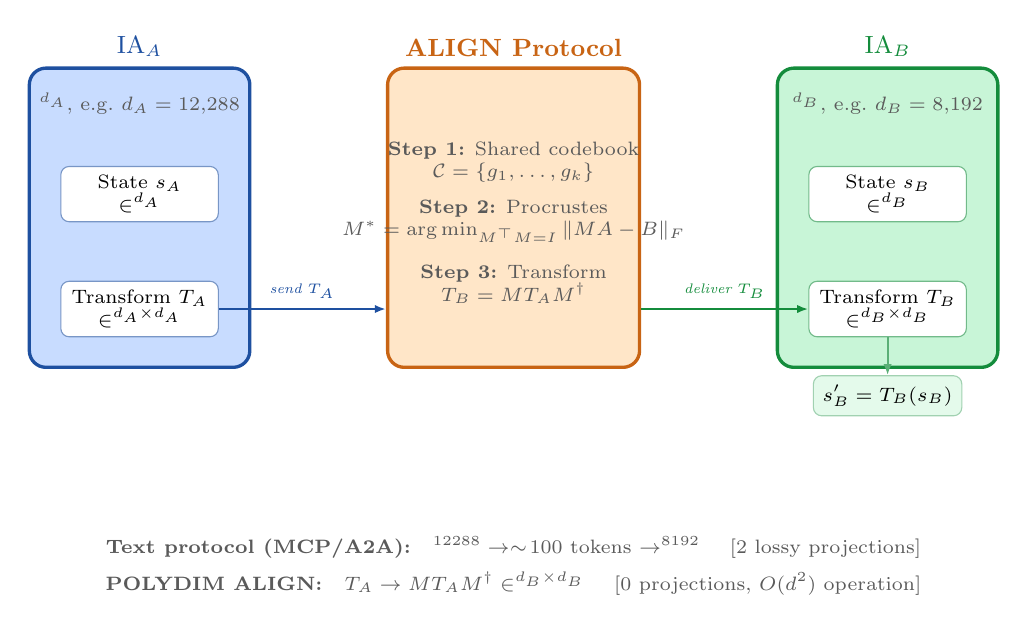
\begin{tikzpicture}[node distance=1.2cm and 2.5cm]

  %% IA_A box
  \node[draw=polyblue, fill=polylightblue, rounded corners=6pt,
        minimum width=2.8cm, minimum height=3.8cm, line width=1.2pt]
    (IA_A) at (0, 0) {};
  \node[above=0pt of IA_A.north, font=\small\bfseries\color{polyblue}]
    {$\mathrm{IA}_A$};
  \node[below=6pt of IA_A.north, font=\scriptsize\color{polygray}]
    {$\RR^{d_A}$, e.g.\ $d_A = 12{,}288$};

  \node[draw=polyblue!60, fill=white, rounded corners=3pt,
        minimum width=2.0cm, font=\scriptsize, align=center]
    (stateA) at (0, 0.3) {State $s_A$\\$\in \RR^{d_A}$};
  \node[draw=polyblue!60, fill=white, rounded corners=3pt,
        minimum width=2.0cm, font=\scriptsize, align=center,
        below=0.2cm of stateA]
    (transA) at (0,-0.6) {Transform $T_A$\\$\in \RR^{d_A \times d_A}$};

  %% IA_B box
  \node[draw=polygreen, fill=polylightgreen, rounded corners=6pt,
        minimum width=2.8cm, minimum height=3.8cm, line width=1.2pt]
    (IA_B) at (9.5, 0) {};
  \node[above=0pt of IA_B.north, font=\small\bfseries\color{polygreen}]
    {$\mathrm{IA}_B$};
  \node[below=6pt of IA_B.north, font=\scriptsize\color{polygray}]
    {$\RR^{d_B}$, e.g.\ $d_B = 8{,}192$};

  \node[draw=polygreen!60, fill=white, rounded corners=3pt,
        minimum width=2.0cm, font=\scriptsize, align=center]
    (stateB) at (9.5, 0.3) {State $s_B$\\$\in \RR^{d_B}$};
  \node[draw=polygreen!60, fill=white, rounded corners=3pt,
        minimum width=2.0cm, font=\scriptsize, align=center,
        below=0.2cm of stateB]
    (transB) at (9.5,-0.6) {Transform $T_B$\\$\in \RR^{d_B \times d_B}$};

  %% ALIGN box in the middle
  \node[draw=polyorange, fill=polylightorange, rounded corners=6pt,
        minimum width=3.2cm, minimum height=3.8cm, line width=1.2pt]
    (align) at (4.75, 0) {};
  \node[above=0pt of align.north, font=\small\bfseries\color{polyorange}]
    {ALIGN Protocol};

  \node[font=\scriptsize, align=center, text=polygray]
    at (4.75, 0.7) {
      \textbf{Step 1:} Shared codebook \\
      $\mathcal{C} = \{g_1, \ldots, g_k\}$
    };
  \node[font=\scriptsize, align=center, text=polygray]
    at (4.75, -0.05) {
      \textbf{Step 2:} Procrustes \\
      $M^* = \arg\min_{M^\top M=I} \|MA-B\|_F$
    };
  \node[font=\scriptsize, align=center, text=polygray]
    at (4.75, -0.85) {
      \textbf{Step 3:} Transform \\
      $T_B = M T_A M^\dagger$
    };

  %% Arrows
  \draw[-{Latex[length=4pt]}, polyblue, line width=0.9pt]
    (transA.east) -- node[above, font=\tiny\itshape] {send $T_A$}
    (align.west |- transA.east);

  \draw[-{Latex[length=4pt]}, polygreen, line width=0.9pt]
    (align.east |- transB.west) --
    node[above, font=\tiny\itshape] {deliver $T_B$}
    (transB.west);

  %% Application
  \node[draw=polygreen!40, fill=polylightgreen!50, rounded corners=3pt,
        font=\scriptsize, align=center, below=0.5cm of stateB]
    (apply) at (9.5,-1.5) {$s_B' = T_B(s_B)$};
  \draw[-{Latex[length=4pt]}, polygreen!70, line width=0.7pt]
    (transB.south) -- (apply.north);

  %% Comparison
  \node[below=2.0cm of align.south, anchor=north,
        font=\scriptsize, align=center, text=polygray] {
    \textbf{Text protocol (MCP/A2A):}\quad
    $\RR^{12288} \to \sim\!100$ tokens $\to \RR^{8192}$
    \quad [2 lossy projections] \\[4pt]
    \textbf{POLYDIM ALIGN:}\quad
    $T_A \to M T_A M^\dagger \in \RR^{d_B \times d_B}$
    \quad [0 projections, $O(d^2)$ operation]
  };

\end{tikzpicture}

\bigskip
%% ============================================================
%% FIGURE 4: Dimensional Type System
%% ============================================================
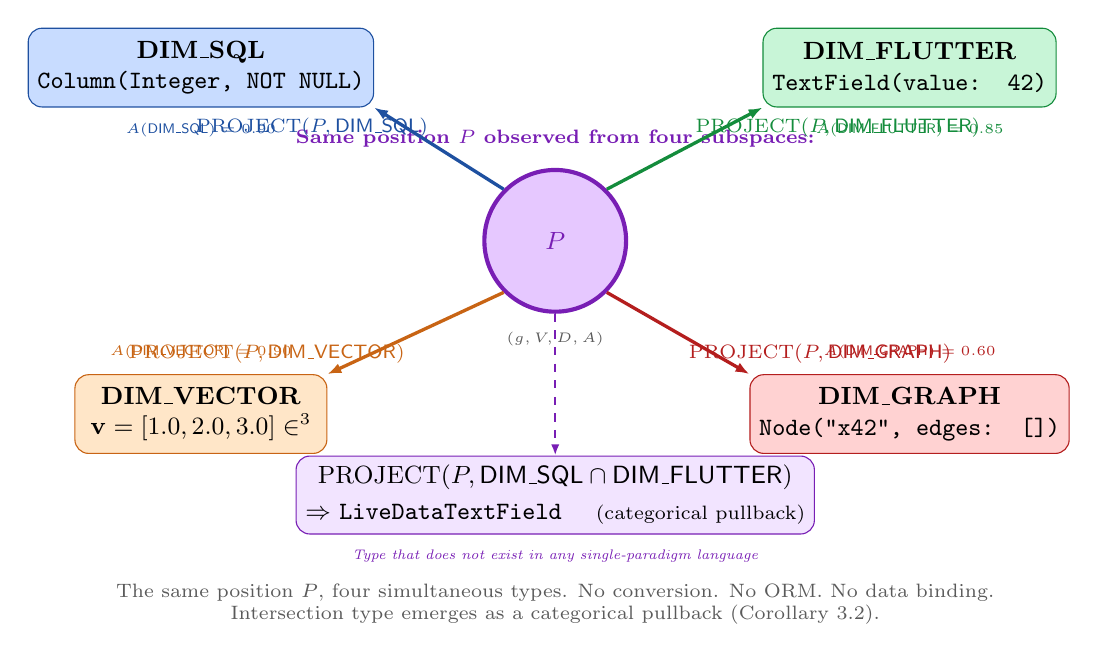
\begin{tikzpicture}[node distance=0.8cm and 1.5cm]

  %% Central position P
  \node[draw=polypurple, fill=polylightpurple, circle,
        minimum size=1.8cm, line width=1.5pt,
        font=\small\bfseries, text=polypurple]
    (P) at (0, 0) {$P$};

  \node[below=3pt of P, font=\tiny\color{polygray}]
    {$(g, V, D, A)$};

  \node[above=4pt of P.north, font=\scriptsize\bfseries, text=polypurple]
    {Same position $P$ observed from four subspaces:};

  %% DIM_SQL projection
  \node[draw=polyblue, fill=polylightblue, rounded corners=5pt,
        minimum width=3.2cm, minimum height=1.0cm,
        font=\small, align=center]
    (sql) at (-4.5, 2.2) {
      \textbf{DIM\_SQL} \\
      \small\texttt{Column(Integer, NOT NULL)}
    };
  \draw[-{Latex[length=5pt]}, polyblue, line width=1.2pt]
    (P.north west) -- node[above left, font=\scriptsize, text=polyblue]
    {$\mathrm{PROJECT}(P, \mathsf{DIM\_SQL})$} (sql.south east);
  \node[below=2pt of sql.south, font=\tiny\itshape, text=polyblue]
    {$A(\mathsf{DIM\_SQL}) = 0.90$};

  %% DIM_FLUTTER projection
  \node[draw=polygreen, fill=polylightgreen, rounded corners=5pt,
        minimum width=3.2cm, minimum height=1.0cm,
        font=\small, align=center]
    (flutter) at (4.5, 2.2) {
      \textbf{DIM\_FLUTTER} \\
      \small\texttt{TextField(value: 42)}
    };
  \draw[-{Latex[length=5pt]}, polygreen, line width=1.2pt]
    (P.north east) -- node[above right, font=\scriptsize, text=polygreen]
    {$\mathrm{PROJECT}(P, \mathsf{DIM\_FLUTTER})$} (flutter.south west);
  \node[below=2pt of flutter.south, font=\tiny\itshape, text=polygreen]
    {$A(\mathsf{DIM\_FLUTTER}) = 0.85$};

  %% DIM_VECTOR projection
  \node[draw=polyorange, fill=polylightorange, rounded corners=5pt,
        minimum width=3.2cm, minimum height=1.0cm,
        font=\small, align=center]
    (vector) at (-4.5, -2.2) {
      \textbf{DIM\_VECTOR} \\
      \small$\mathbf{v} = [1.0, 2.0, 3.0] \in \RR^3$
    };
  \draw[-{Latex[length=5pt]}, polyorange, line width=1.2pt]
    (P.south west) -- node[below left, font=\scriptsize, text=polyorange]
    {$\mathrm{PROJECT}(P, \mathsf{DIM\_VECTOR})$} (vector.north east);
  \node[above=2pt of vector.north, font=\tiny\itshape, text=polyorange]
    {$A(\mathsf{DIM\_VECTOR}) = 0.90$};

  %% DIM_GRAPH projection
  \node[draw=polyred, fill=polylightred, rounded corners=5pt,
        minimum width=3.2cm, minimum height=1.0cm,
        font=\small, align=center]
    (graph) at (4.5, -2.2) {
      \textbf{DIM\_GRAPH} \\
      \small\texttt{Node("x42", edges: [])}
    };
  \draw[-{Latex[length=5pt]}, polyred, line width=1.2pt]
    (P.south east) -- node[below right, font=\scriptsize, text=polyred]
    {$\mathrm{PROJECT}(P, \mathsf{DIM\_GRAPH})$} (graph.north west);
  \node[above=2pt of graph.north, font=\tiny\itshape, text=polyred]
    {$A(\mathsf{DIM\_GRAPH}) = 0.60$};

  %% Intersection type (pullback)
  \node[draw=polypurple, fill=polylightpurple!50, rounded corners=5pt,
        minimum width=4.0cm, minimum height=0.9cm,
        font=\small, align=center, below=1.8cm of P]
    (intersect) {
      $\mathrm{PROJECT}(P, \mathsf{DIM\_SQL} \cap \mathsf{DIM\_FLUTTER})$ \\[2pt]
      \small $\Rightarrow$ \texttt{LiveDataTextField} \quad
      \scriptsize(categorical pullback)
    };
  \draw[-{Latex[length=4pt]}, polypurple, dashed, line width=0.9pt]
    (P.south) -- (intersect.north);
  \node[below=2pt of intersect.south, font=\tiny\itshape, text=polypurple]
    {Type that does not exist in any single-paradigm language};

  %% Caption
  \node[below=0.5cm of intersect.south, anchor=north,
        font=\scriptsize, text=polygray, align=center] {
    The same position $P$, four simultaneous types. No conversion. No ORM. No data binding. \\
    Intersection type emerges as a categorical pullback (Corollary~3.2).
  };

\end{tikzpicture}

\end{document}
 en polydim_paper_arxiv.tex
%          O compilar standalone con pdflatex para preview
%
% Figuras incluidas:
%   Fig 1: PROJECT como funtor (G → E_X)
%   Fig 2: Arquitectura dos capas (Algebraic / Implementation)
%   Fig 3: Protocolo ALIGN AI↔AI
%   Fig 4: Sistema de tipos dimensional (el mismo objeto, 4 proyecciones)

\documentclass[tikz,border=6pt]{standalone}
\usepackage{tikz}
\usepackage{amsmath,amssymb}
\usepackage{xcolor}
\usetikzlibrary{
  arrows.meta,
  positioning,
  shapes.geometric,
  shapes.misc,
  fit,
  backgrounds,
  decorations.pathreplacing,
  matrix,
  calc,
  shadows.blur
}

%% ============================================================
%% Color palette
%% ============================================================
\definecolor{polyblue}{RGB}{30,80,160}
\definecolor{polylightblue}{RGB}{200,220,255}
\definecolor{polygreen}{RGB}{20,140,60}
\definecolor{polylightgreen}{RGB}{200,245,215}
\definecolor{polyorange}{RGB}{200,100,20}
\definecolor{polylightorange}{RGB}{255,230,200}
\definecolor{polyred}{RGB}{180,30,30}
\definecolor{polylightred}{RGB}{255,210,210}
\definecolor{polygray}{RGB}{90,90,90}
\definecolor{polylightgray}{RGB}{240,240,240}
\definecolor{polypurple}{RGB}{120,30,180}
\definecolor{polylightpurple}{RGB}{230,200,255}

%% ============================================================
%% Common TikZ styles
%% ============================================================
\tikzset{
  %% Category box
  catbox/.style={
    draw=#1, fill=#1!10, rounded corners=6pt,
    minimum width=3.2cm, minimum height=2.4cm,
    line width=1.2pt, font=\small
  },
  %% Object node
  objnode/.style={
    draw=#1, fill=#1!20, circle,
    minimum size=0.55cm, line width=0.8pt,
    font=\scriptsize\bfseries, text=#1!60!black
  },
  %% Morphism arrow
  morpharrow/.style={
    -{Latex[length=4pt,width=3pt]},
    draw=#1, line width=0.9pt
  },
  %% Functor arrow
  functarrow/.style={
    -{Latex[length=6pt,width=5pt]},
    draw=polyorange, line width=1.8pt,
    double=polylightorange, double distance=1.5pt
  },
  %% Layer box
  layerbox/.style={
    draw=#1, fill=#1!8, rounded corners=4pt,
    minimum width=8cm, line width=1.2pt,
    font=\small\bfseries, text=#1
  },
  %% Primitive node
  primnode/.style={
    draw=#1, fill=#1!15, rounded corners=3pt,
    minimum width=2.6cm, minimum height=0.65cm,
    line width=0.8pt, font=\small
  },
}

\begin{document}

%% ============================================================
%% FIGURE 1: PROJECT as a Functor  G → E_X
%% ============================================================
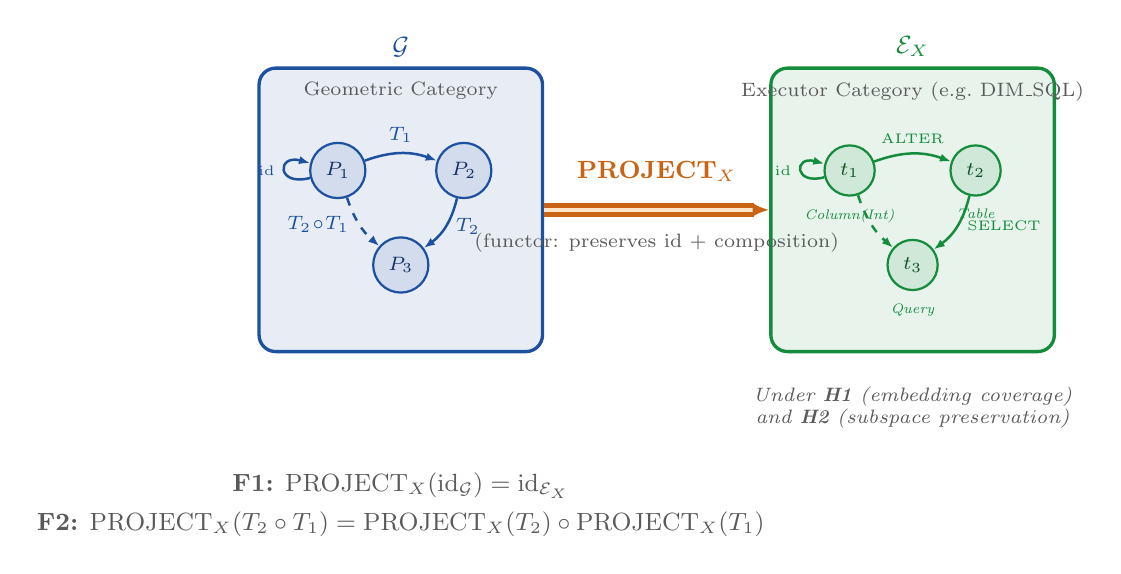
\begin{tikzpicture}[node distance=1cm and 3.8cm]

  %% ── Geometric category G ─────────────────────────────────
  \node[catbox=polyblue, minimum width=3.6cm, minimum height=3.6cm]
    (Gbox) at (0,0) {};
  \node[above=0pt of Gbox.north, font=\small\bfseries\color{polyblue}]
    {$\mathcal{G}$};
  \node[below=2pt of Gbox.north, font=\scriptsize\color{polygray}]
    {Geometric Category};

  % Objects in G
  \node[objnode=polyblue] (P1) at (-0.8, 0.5) {$P_1$};
  \node[objnode=polyblue] (P2) at ( 0.8, 0.5) {$P_2$};
  \node[objnode=polyblue] (P3) at ( 0.0,-0.7) {$P_3$};

  % Morphisms in G (transformations T)
  \draw[morpharrow=polyblue]
    (P1) to[bend left=20]
    node[above, font=\scriptsize, text=polyblue] {$T_1$} (P2);
  \draw[morpharrow=polyblue]
    (P2) to[bend left=20]
    node[right, font=\scriptsize, text=polyblue] {$T_2$} (P3);
  \draw[morpharrow=polyblue, dashed]
    (P1) to[bend right=15]
    node[left, font=\scriptsize, text=polyblue] {$T_2\!\circ\!T_1$} (P3);

  % Identity
  \draw[morpharrow=polyblue]
    (P1) to[loop left, looseness=6]
    node[left, font=\tiny, text=polyblue] {$\mathrm{id}$} (P1);

  %% ── Executor category E_X ────────────────────────────────
  \node[catbox=polygreen, minimum width=3.6cm, minimum height=3.6cm]
    (Ebox) at (6.5, 0) {};
  \node[above=0pt of Ebox.north, font=\small\bfseries\color{polygreen}]
    {$\mathcal{E}_X$};
  \node[below=2pt of Ebox.north, font=\scriptsize\color{polygray}]
    {Executor Category (e.g.\ DIM\_SQL)};

  % Objects in E_X (types)
  \node[objnode=polygreen] (t1) at (5.7, 0.5)
    {\scriptsize $t_1$};
  \node[objnode=polygreen] (t2) at (7.3, 0.5)
    {\scriptsize $t_2$};
  \node[objnode=polygreen] (t3) at (6.5,-0.7)
    {\scriptsize $t_3$};

  % Type labels
  \node[below=1pt of t1, font=\tiny\itshape, text=polygreen]
    {Column(Int)};
  \node[below=1pt of t2, font=\tiny\itshape, text=polygreen]
    {Table};
  \node[below=1pt of t3, font=\tiny\itshape, text=polygreen]
    {Query};

  % Morphisms in E_X (type maps)
  \draw[morpharrow=polygreen]
    (t1) to[bend left=20]
    node[above, font=\tiny, text=polygreen] {ALTER} (t2);
  \draw[morpharrow=polygreen]
    (t2) to[bend left=20]
    node[right, font=\tiny, text=polygreen] {SELECT} (t3);
  \draw[morpharrow=polygreen, dashed]
    (t1) to[bend right=15]
    node[left, font=\tiny, text=polygreen] {} (t3);

  \draw[morpharrow=polygreen]
    (t1) to[loop left, looseness=6]
    node[left, font=\tiny, text=polygreen] {$\mathrm{id}$} (t1);

  %% ── PROJECT_X functor arrow ───────────────────────────────
  \draw[functarrow]
    ($(Gbox.east)+(0,0)$) -- node[above=6pt, font=\small\bfseries\color{polyorange}]
    {$\mathbf{PROJECT}_X$}
    node[below=4pt, font=\scriptsize\color{polygray}]
    {(functor: preserves id + composition)}
    ($(Ebox.west)+(0,0)$);

  %% ── Functor equations ────────────────────────────────────
  \node[below=1.4cm of Gbox.south, anchor=north,
        font=\small, text=polygray, align=center] {
    \textbf{F1:} $\mathrm{PROJECT}_X(\mathrm{id}_\mathcal{G}) = \mathrm{id}_{\mathcal{E}_X}$ \\[3pt]
    \textbf{F2:} $\mathrm{PROJECT}_X(T_2 \circ T_1) =
                  \mathrm{PROJECT}_X(T_2) \circ \mathrm{PROJECT}_X(T_1)$
  };

  %% ── H2 annotation ────────────────────────────────────────
  \node[below=0.3cm of Ebox.south, anchor=north,
        font=\scriptsize\itshape, text=polygray, align=center] {
    Under \textbf{H1} (embedding coverage) \\
    and \textbf{H2} (subspace preservation)
  };

\end{tikzpicture}

\bigskip
%% ============================================================
%% FIGURE 2: Two-Layer Architecture
%% ============================================================
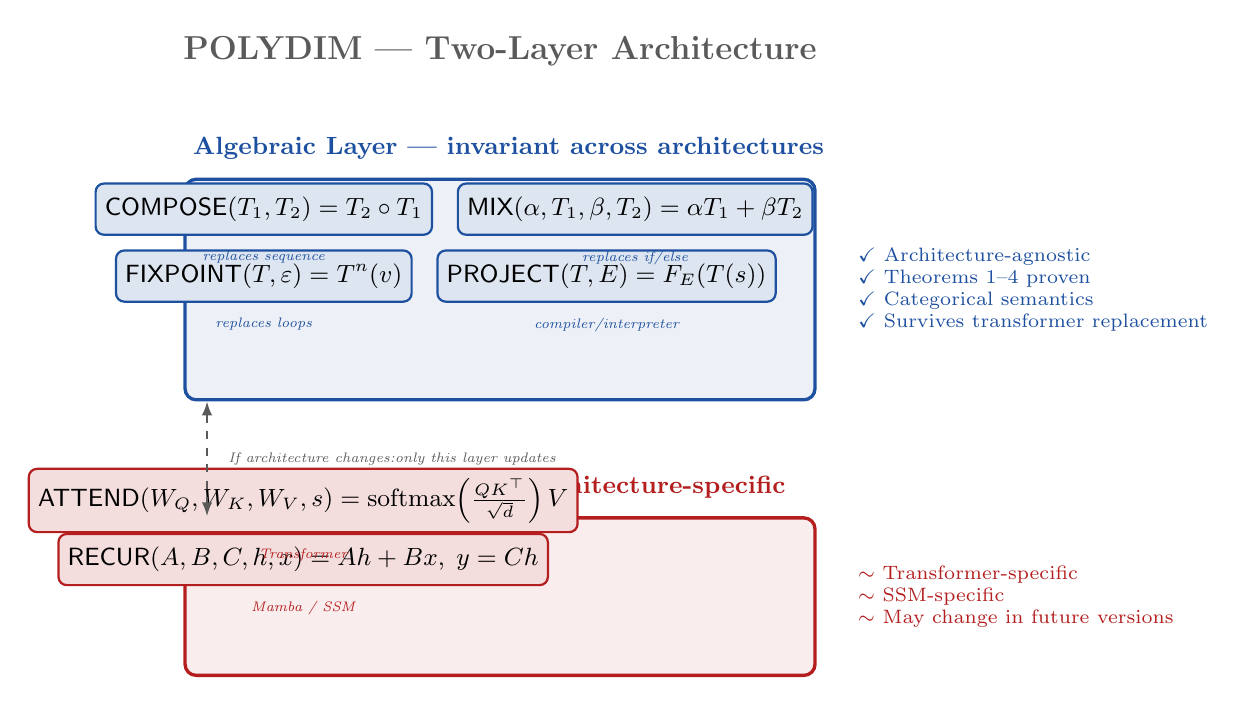
\begin{tikzpicture}[node distance=0.5cm]

  %% Title
  \node[font=\large\bfseries, text=polygray] (title) at (4, 0)
    {POLYDIM — Two-Layer Architecture};

  %% ── ALGEBRAIC LAYER ──────────────────────────────────────
  \node[layerbox=polyblue, minimum height=2.8cm,
        below=0.8cm of title, anchor=north] (alglayer) at (4, -0.8) {};

  \node[above=3pt of alglayer.north west, anchor=south west,
        font=\small\bfseries, text=polyblue]
    {Algebraic Layer — invariant across architectures};

  % Primitives
  \node[primnode=polyblue] (compose) at (1.0,-2.0)
    {$\mathsf{COMPOSE}(T_1, T_2) = T_2 \circ T_1$};
  \node[primnode=polyblue, right=0.3cm of compose] (mix)
    {$\mathsf{MIX}(\alpha, T_1, \beta, T_2) = \alpha T_1 + \beta T_2$};
  \node[primnode=polyblue] (fix) at (1.0,-2.85)
    {$\mathsf{FIXPOINT}(T, \varepsilon) = T^n(v)$};
  \node[primnode=polyblue, right=0.3cm of fix] (proj)
    {$\mathsf{PROJECT}(T, E) = F_E(T(s))$};

  % Property tags
  \node[below=2pt of compose.south, font=\tiny\itshape, text=polyblue]
    {replaces sequence};
  \node[below=2pt of mix.south, font=\tiny\itshape, text=polyblue]
    {replaces if/else};
  \node[below=2pt of fix.south, font=\tiny\itshape, text=polyblue]
    {replaces loops};
  \node[below=2pt of proj.south, font=\tiny\itshape, text=polyblue]
    {compiler/interpreter};

  %% ── IMPLEMENTATION LAYER ─────────────────────────────────
  \node[layerbox=polyred, minimum height=2.0cm,
        below=1.1cm of alglayer.south, anchor=north] (impllayer) at (4,-4.8) {};

  \node[above=3pt of impllayer.north west, anchor=south west,
        font=\small\bfseries, text=polyred]
    {Implementation Layer — architecture-specific};

  \node[primnode=polyred] (attend) at (1.5,-5.7)
    {$\mathsf{ATTEND}(W_Q, W_K, W_V, s) = \mathrm{softmax}\!\left(\tfrac{QK^\top}{\sqrt{d}}\right)V$};
  \node[primnode=polyred] (recur) at (1.5,-6.45)
    {$\mathsf{RECUR}(A, B, C, h, x) = Ah + Bx,\; y = Ch$};

  \node[below=2pt of attend.south, font=\tiny\itshape, text=polyred]
    {Transformer};
  \node[below=2pt of recur.south, font=\tiny\itshape, text=polyred]
    {Mamba / SSM};

  %% ── Separator arrow ──────────────────────────────────────
  \draw[{Latex[length=5pt]}-{Latex[length=5pt]},
        draw=polygray, dashed, line width=0.7pt]
    ($(alglayer.south west)+(0.3,0)$) --
    node[right=4pt, font=\tiny\itshape, text=polygray]
      {If architecture changes:\\
       only this layer updates}
    ($(impllayer.north west)+(0.3,0)$);

  %% ── Property annotations ─────────────────────────────────
  \node[right=0.4cm of alglayer.east, anchor=west,
        font=\scriptsize, text=polyblue, align=left] {
    \checkmark\ Architecture-agnostic \\
    \checkmark\ Theorems 1--4 proven \\
    \checkmark\ Categorical semantics \\
    \checkmark\ Survives transformer replacement
  };

  \node[right=0.4cm of impllayer.east, anchor=west,
        font=\scriptsize, text=polyred, align=left] {
    $\sim$\ Transformer-specific \\
    $\sim$\ SSM-specific \\
    $\sim$\ May change in future versions
  };

\end{tikzpicture}

\bigskip
%% ============================================================
%% FIGURE 3: ALIGN Protocol — AI-to-AI Communication
%% ============================================================
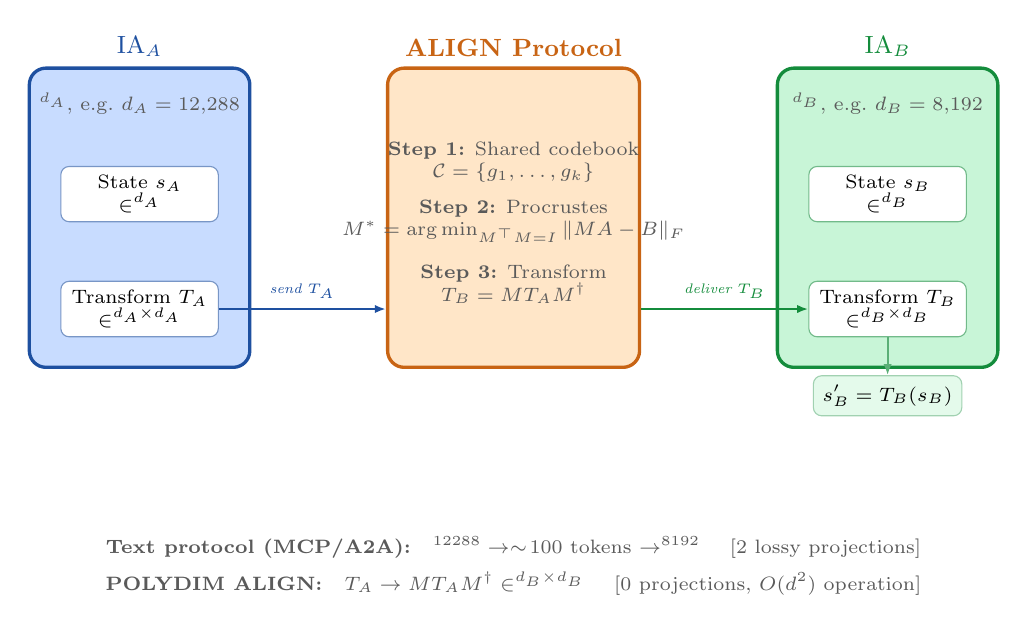
\begin{tikzpicture}[node distance=1.2cm and 2.5cm]

  %% IA_A box
  \node[draw=polyblue, fill=polylightblue, rounded corners=6pt,
        minimum width=2.8cm, minimum height=3.8cm, line width=1.2pt]
    (IA_A) at (0, 0) {};
  \node[above=0pt of IA_A.north, font=\small\bfseries\color{polyblue}]
    {$\mathrm{IA}_A$};
  \node[below=6pt of IA_A.north, font=\scriptsize\color{polygray}]
    {$\RR^{d_A}$, e.g.\ $d_A = 12{,}288$};

  \node[draw=polyblue!60, fill=white, rounded corners=3pt,
        minimum width=2.0cm, font=\scriptsize, align=center]
    (stateA) at (0, 0.3) {State $s_A$\\$\in \RR^{d_A}$};
  \node[draw=polyblue!60, fill=white, rounded corners=3pt,
        minimum width=2.0cm, font=\scriptsize, align=center,
        below=0.2cm of stateA]
    (transA) at (0,-0.6) {Transform $T_A$\\$\in \RR^{d_A \times d_A}$};

  %% IA_B box
  \node[draw=polygreen, fill=polylightgreen, rounded corners=6pt,
        minimum width=2.8cm, minimum height=3.8cm, line width=1.2pt]
    (IA_B) at (9.5, 0) {};
  \node[above=0pt of IA_B.north, font=\small\bfseries\color{polygreen}]
    {$\mathrm{IA}_B$};
  \node[below=6pt of IA_B.north, font=\scriptsize\color{polygray}]
    {$\RR^{d_B}$, e.g.\ $d_B = 8{,}192$};

  \node[draw=polygreen!60, fill=white, rounded corners=3pt,
        minimum width=2.0cm, font=\scriptsize, align=center]
    (stateB) at (9.5, 0.3) {State $s_B$\\$\in \RR^{d_B}$};
  \node[draw=polygreen!60, fill=white, rounded corners=3pt,
        minimum width=2.0cm, font=\scriptsize, align=center,
        below=0.2cm of stateB]
    (transB) at (9.5,-0.6) {Transform $T_B$\\$\in \RR^{d_B \times d_B}$};

  %% ALIGN box in the middle
  \node[draw=polyorange, fill=polylightorange, rounded corners=6pt,
        minimum width=3.2cm, minimum height=3.8cm, line width=1.2pt]
    (align) at (4.75, 0) {};
  \node[above=0pt of align.north, font=\small\bfseries\color{polyorange}]
    {ALIGN Protocol};

  \node[font=\scriptsize, align=center, text=polygray]
    at (4.75, 0.7) {
      \textbf{Step 1:} Shared codebook \\
      $\mathcal{C} = \{g_1, \ldots, g_k\}$
    };
  \node[font=\scriptsize, align=center, text=polygray]
    at (4.75, -0.05) {
      \textbf{Step 2:} Procrustes \\
      $M^* = \arg\min_{M^\top M=I} \|MA-B\|_F$
    };
  \node[font=\scriptsize, align=center, text=polygray]
    at (4.75, -0.85) {
      \textbf{Step 3:} Transform \\
      $T_B = M T_A M^\dagger$
    };

  %% Arrows
  \draw[-{Latex[length=4pt]}, polyblue, line width=0.9pt]
    (transA.east) -- node[above, font=\tiny\itshape] {send $T_A$}
    (align.west |- transA.east);

  \draw[-{Latex[length=4pt]}, polygreen, line width=0.9pt]
    (align.east |- transB.west) --
    node[above, font=\tiny\itshape] {deliver $T_B$}
    (transB.west);

  %% Application
  \node[draw=polygreen!40, fill=polylightgreen!50, rounded corners=3pt,
        font=\scriptsize, align=center, below=0.5cm of stateB]
    (apply) at (9.5,-1.5) {$s_B' = T_B(s_B)$};
  \draw[-{Latex[length=4pt]}, polygreen!70, line width=0.7pt]
    (transB.south) -- (apply.north);

  %% Comparison
  \node[below=2.0cm of align.south, anchor=north,
        font=\scriptsize, align=center, text=polygray] {
    \textbf{Text protocol (MCP/A2A):}\quad
    $\RR^{12288} \to \sim\!100$ tokens $\to \RR^{8192}$
    \quad [2 lossy projections] \\[4pt]
    \textbf{POLYDIM ALIGN:}\quad
    $T_A \to M T_A M^\dagger \in \RR^{d_B \times d_B}$
    \quad [0 projections, $O(d^2)$ operation]
  };

\end{tikzpicture}

\bigskip
%% ============================================================
%% FIGURE 4: Dimensional Type System
%% ============================================================
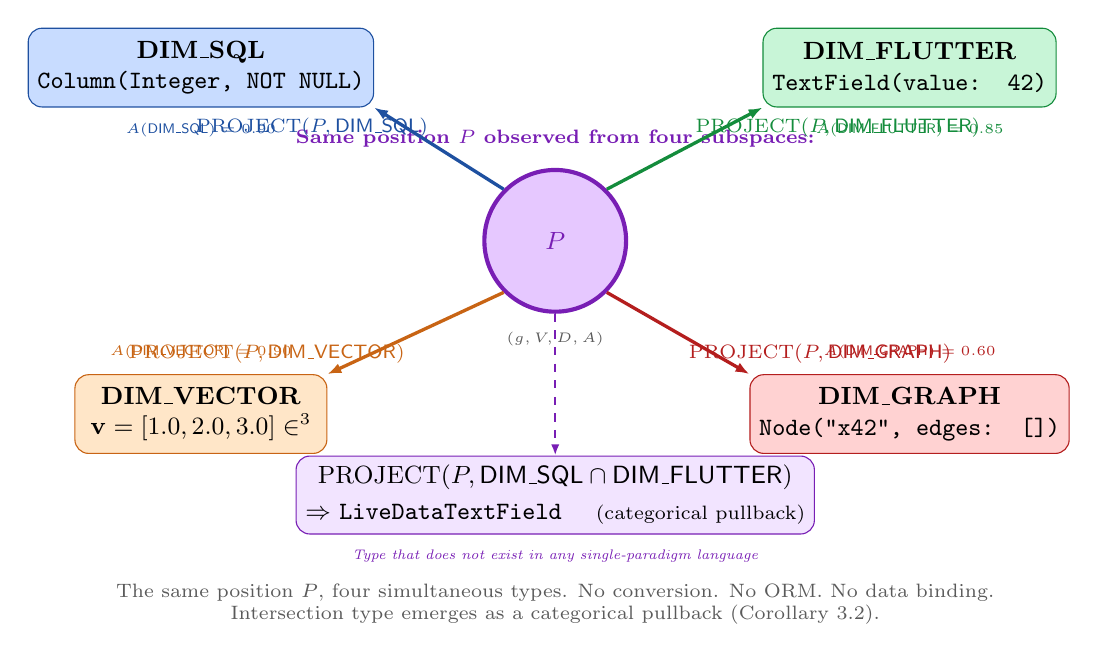
\begin{tikzpicture}[node distance=0.8cm and 1.5cm]

  %% Central position P
  \node[draw=polypurple, fill=polylightpurple, circle,
        minimum size=1.8cm, line width=1.5pt,
        font=\small\bfseries, text=polypurple]
    (P) at (0, 0) {$P$};

  \node[below=3pt of P, font=\tiny\color{polygray}]
    {$(g, V, D, A)$};

  \node[above=4pt of P.north, font=\scriptsize\bfseries, text=polypurple]
    {Same position $P$ observed from four subspaces:};

  %% DIM_SQL projection
  \node[draw=polyblue, fill=polylightblue, rounded corners=5pt,
        minimum width=3.2cm, minimum height=1.0cm,
        font=\small, align=center]
    (sql) at (-4.5, 2.2) {
      \textbf{DIM\_SQL} \\
      \small\texttt{Column(Integer, NOT NULL)}
    };
  \draw[-{Latex[length=5pt]}, polyblue, line width=1.2pt]
    (P.north west) -- node[above left, font=\scriptsize, text=polyblue]
    {$\mathrm{PROJECT}(P, \mathsf{DIM\_SQL})$} (sql.south east);
  \node[below=2pt of sql.south, font=\tiny\itshape, text=polyblue]
    {$A(\mathsf{DIM\_SQL}) = 0.90$};

  %% DIM_FLUTTER projection
  \node[draw=polygreen, fill=polylightgreen, rounded corners=5pt,
        minimum width=3.2cm, minimum height=1.0cm,
        font=\small, align=center]
    (flutter) at (4.5, 2.2) {
      \textbf{DIM\_FLUTTER} \\
      \small\texttt{TextField(value: 42)}
    };
  \draw[-{Latex[length=5pt]}, polygreen, line width=1.2pt]
    (P.north east) -- node[above right, font=\scriptsize, text=polygreen]
    {$\mathrm{PROJECT}(P, \mathsf{DIM\_FLUTTER})$} (flutter.south west);
  \node[below=2pt of flutter.south, font=\tiny\itshape, text=polygreen]
    {$A(\mathsf{DIM\_FLUTTER}) = 0.85$};

  %% DIM_VECTOR projection
  \node[draw=polyorange, fill=polylightorange, rounded corners=5pt,
        minimum width=3.2cm, minimum height=1.0cm,
        font=\small, align=center]
    (vector) at (-4.5, -2.2) {
      \textbf{DIM\_VECTOR} \\
      \small$\mathbf{v} = [1.0, 2.0, 3.0] \in \RR^3$
    };
  \draw[-{Latex[length=5pt]}, polyorange, line width=1.2pt]
    (P.south west) -- node[below left, font=\scriptsize, text=polyorange]
    {$\mathrm{PROJECT}(P, \mathsf{DIM\_VECTOR})$} (vector.north east);
  \node[above=2pt of vector.north, font=\tiny\itshape, text=polyorange]
    {$A(\mathsf{DIM\_VECTOR}) = 0.90$};

  %% DIM_GRAPH projection
  \node[draw=polyred, fill=polylightred, rounded corners=5pt,
        minimum width=3.2cm, minimum height=1.0cm,
        font=\small, align=center]
    (graph) at (4.5, -2.2) {
      \textbf{DIM\_GRAPH} \\
      \small\texttt{Node("x42", edges: [])}
    };
  \draw[-{Latex[length=5pt]}, polyred, line width=1.2pt]
    (P.south east) -- node[below right, font=\scriptsize, text=polyred]
    {$\mathrm{PROJECT}(P, \mathsf{DIM\_GRAPH})$} (graph.north west);
  \node[above=2pt of graph.north, font=\tiny\itshape, text=polyred]
    {$A(\mathsf{DIM\_GRAPH}) = 0.60$};

  %% Intersection type (pullback)
  \node[draw=polypurple, fill=polylightpurple!50, rounded corners=5pt,
        minimum width=4.0cm, minimum height=0.9cm,
        font=\small, align=center, below=1.8cm of P]
    (intersect) {
      $\mathrm{PROJECT}(P, \mathsf{DIM\_SQL} \cap \mathsf{DIM\_FLUTTER})$ \\[2pt]
      \small $\Rightarrow$ \texttt{LiveDataTextField} \quad
      \scriptsize(categorical pullback)
    };
  \draw[-{Latex[length=4pt]}, polypurple, dashed, line width=0.9pt]
    (P.south) -- (intersect.north);
  \node[below=2pt of intersect.south, font=\tiny\itshape, text=polypurple]
    {Type that does not exist in any single-paradigm language};

  %% Caption
  \node[below=0.5cm of intersect.south, anchor=north,
        font=\scriptsize, text=polygray, align=center] {
    The same position $P$, four simultaneous types. No conversion. No ORM. No data binding. \\
    Intersection type emerges as a categorical pullback (Corollary~3.2).
  };

\end{tikzpicture}

\end{document}
 en polydim_paper_arxiv.tex
%          O compilar standalone con pdflatex para preview
%
% Figuras incluidas:
%   Fig 1: PROJECT como funtor (G → E_X)
%   Fig 2: Arquitectura dos capas (Algebraic / Implementation)
%   Fig 3: Protocolo ALIGN AI↔AI
%   Fig 4: Sistema de tipos dimensional (el mismo objeto, 4 proyecciones)

\documentclass[tikz,border=6pt]{standalone}
\usepackage{tikz}
\usepackage{amsmath,amssymb}
\usepackage{xcolor}
\usetikzlibrary{
  arrows.meta,
  positioning,
  shapes.geometric,
  shapes.misc,
  fit,
  backgrounds,
  decorations.pathreplacing,
  matrix,
  calc,
  shadows.blur
}

%% ============================================================
%% Color palette
%% ============================================================
\definecolor{polyblue}{RGB}{30,80,160}
\definecolor{polylightblue}{RGB}{200,220,255}
\definecolor{polygreen}{RGB}{20,140,60}
\definecolor{polylightgreen}{RGB}{200,245,215}
\definecolor{polyorange}{RGB}{200,100,20}
\definecolor{polylightorange}{RGB}{255,230,200}
\definecolor{polyred}{RGB}{180,30,30}
\definecolor{polylightred}{RGB}{255,210,210}
\definecolor{polygray}{RGB}{90,90,90}
\definecolor{polylightgray}{RGB}{240,240,240}
\definecolor{polypurple}{RGB}{120,30,180}
\definecolor{polylightpurple}{RGB}{230,200,255}

%% ============================================================
%% Common TikZ styles
%% ============================================================
\tikzset{
  %% Category box
  catbox/.style={
    draw=#1, fill=#1!10, rounded corners=6pt,
    minimum width=3.2cm, minimum height=2.4cm,
    line width=1.2pt, font=\small
  },
  %% Object node
  objnode/.style={
    draw=#1, fill=#1!20, circle,
    minimum size=0.55cm, line width=0.8pt,
    font=\scriptsize\bfseries, text=#1!60!black
  },
  %% Morphism arrow
  morpharrow/.style={
    -{Latex[length=4pt,width=3pt]},
    draw=#1, line width=0.9pt
  },
  %% Functor arrow
  functarrow/.style={
    -{Latex[length=6pt,width=5pt]},
    draw=polyorange, line width=1.8pt,
    double=polylightorange, double distance=1.5pt
  },
  %% Layer box
  layerbox/.style={
    draw=#1, fill=#1!8, rounded corners=4pt,
    minimum width=8cm, line width=1.2pt,
    font=\small\bfseries, text=#1
  },
  %% Primitive node
  primnode/.style={
    draw=#1, fill=#1!15, rounded corners=3pt,
    minimum width=2.6cm, minimum height=0.65cm,
    line width=0.8pt, font=\small
  },
}

\begin{document}

%% ============================================================
%% FIGURE 1: PROJECT as a Functor  G → E_X
%% ============================================================
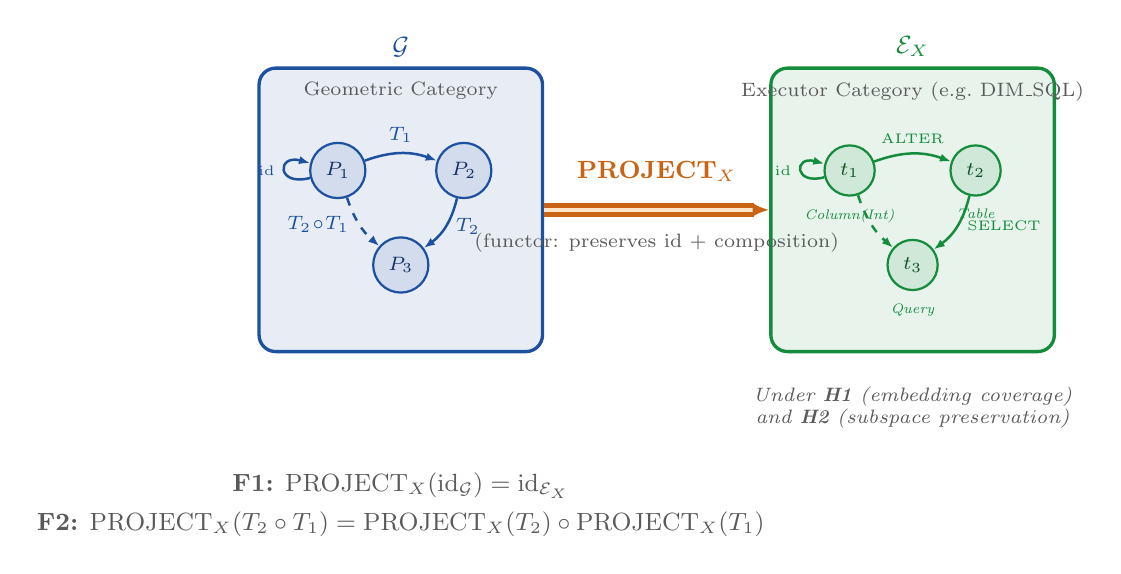
\begin{tikzpicture}[node distance=1cm and 3.8cm]

  %% ── Geometric category G ─────────────────────────────────
  \node[catbox=polyblue, minimum width=3.6cm, minimum height=3.6cm]
    (Gbox) at (0,0) {};
  \node[above=0pt of Gbox.north, font=\small\bfseries\color{polyblue}]
    {$\mathcal{G}$};
  \node[below=2pt of Gbox.north, font=\scriptsize\color{polygray}]
    {Geometric Category};

  % Objects in G
  \node[objnode=polyblue] (P1) at (-0.8, 0.5) {$P_1$};
  \node[objnode=polyblue] (P2) at ( 0.8, 0.5) {$P_2$};
  \node[objnode=polyblue] (P3) at ( 0.0,-0.7) {$P_3$};

  % Morphisms in G (transformations T)
  \draw[morpharrow=polyblue]
    (P1) to[bend left=20]
    node[above, font=\scriptsize, text=polyblue] {$T_1$} (P2);
  \draw[morpharrow=polyblue]
    (P2) to[bend left=20]
    node[right, font=\scriptsize, text=polyblue] {$T_2$} (P3);
  \draw[morpharrow=polyblue, dashed]
    (P1) to[bend right=15]
    node[left, font=\scriptsize, text=polyblue] {$T_2\!\circ\!T_1$} (P3);

  % Identity
  \draw[morpharrow=polyblue]
    (P1) to[loop left, looseness=6]
    node[left, font=\tiny, text=polyblue] {$\mathrm{id}$} (P1);

  %% ── Executor category E_X ────────────────────────────────
  \node[catbox=polygreen, minimum width=3.6cm, minimum height=3.6cm]
    (Ebox) at (6.5, 0) {};
  \node[above=0pt of Ebox.north, font=\small\bfseries\color{polygreen}]
    {$\mathcal{E}_X$};
  \node[below=2pt of Ebox.north, font=\scriptsize\color{polygray}]
    {Executor Category (e.g.\ DIM\_SQL)};

  % Objects in E_X (types)
  \node[objnode=polygreen] (t1) at (5.7, 0.5)
    {\scriptsize $t_1$};
  \node[objnode=polygreen] (t2) at (7.3, 0.5)
    {\scriptsize $t_2$};
  \node[objnode=polygreen] (t3) at (6.5,-0.7)
    {\scriptsize $t_3$};

  % Type labels
  \node[below=1pt of t1, font=\tiny\itshape, text=polygreen]
    {Column(Int)};
  \node[below=1pt of t2, font=\tiny\itshape, text=polygreen]
    {Table};
  \node[below=1pt of t3, font=\tiny\itshape, text=polygreen]
    {Query};

  % Morphisms in E_X (type maps)
  \draw[morpharrow=polygreen]
    (t1) to[bend left=20]
    node[above, font=\tiny, text=polygreen] {ALTER} (t2);
  \draw[morpharrow=polygreen]
    (t2) to[bend left=20]
    node[right, font=\tiny, text=polygreen] {SELECT} (t3);
  \draw[morpharrow=polygreen, dashed]
    (t1) to[bend right=15]
    node[left, font=\tiny, text=polygreen] {} (t3);

  \draw[morpharrow=polygreen]
    (t1) to[loop left, looseness=6]
    node[left, font=\tiny, text=polygreen] {$\mathrm{id}$} (t1);

  %% ── PROJECT_X functor arrow ───────────────────────────────
  \draw[functarrow]
    ($(Gbox.east)+(0,0)$) -- node[above=6pt, font=\small\bfseries\color{polyorange}]
    {$\mathbf{PROJECT}_X$}
    node[below=4pt, font=\scriptsize\color{polygray}]
    {(functor: preserves id + composition)}
    ($(Ebox.west)+(0,0)$);

  %% ── Functor equations ────────────────────────────────────
  \node[below=1.4cm of Gbox.south, anchor=north,
        font=\small, text=polygray, align=center] {
    \textbf{F1:} $\mathrm{PROJECT}_X(\mathrm{id}_\mathcal{G}) = \mathrm{id}_{\mathcal{E}_X}$ \\[3pt]
    \textbf{F2:} $\mathrm{PROJECT}_X(T_2 \circ T_1) =
                  \mathrm{PROJECT}_X(T_2) \circ \mathrm{PROJECT}_X(T_1)$
  };

  %% ── H2 annotation ────────────────────────────────────────
  \node[below=0.3cm of Ebox.south, anchor=north,
        font=\scriptsize\itshape, text=polygray, align=center] {
    Under \textbf{H1} (embedding coverage) \\
    and \textbf{H2} (subspace preservation)
  };

\end{tikzpicture}

\bigskip
%% ============================================================
%% FIGURE 2: Two-Layer Architecture
%% ============================================================
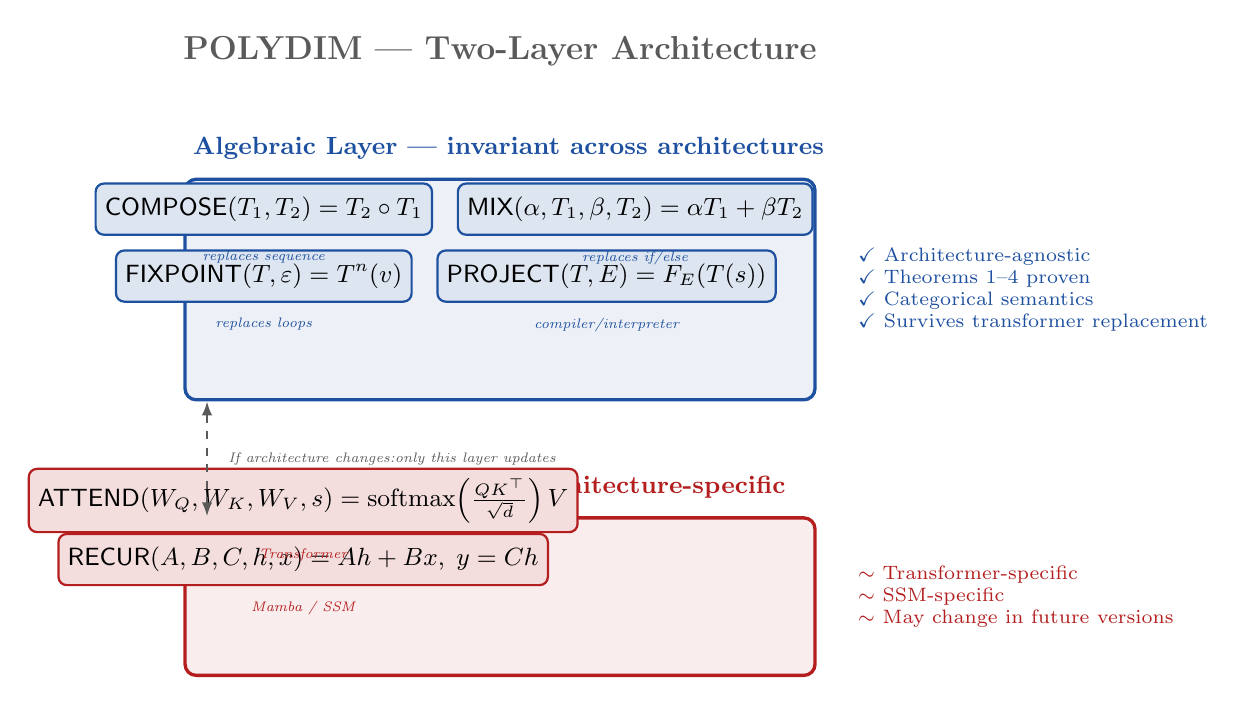
\begin{tikzpicture}[node distance=0.5cm]

  %% Title
  \node[font=\large\bfseries, text=polygray] (title) at (4, 0)
    {POLYDIM — Two-Layer Architecture};

  %% ── ALGEBRAIC LAYER ──────────────────────────────────────
  \node[layerbox=polyblue, minimum height=2.8cm,
        below=0.8cm of title, anchor=north] (alglayer) at (4, -0.8) {};

  \node[above=3pt of alglayer.north west, anchor=south west,
        font=\small\bfseries, text=polyblue]
    {Algebraic Layer — invariant across architectures};

  % Primitives
  \node[primnode=polyblue] (compose) at (1.0,-2.0)
    {$\mathsf{COMPOSE}(T_1, T_2) = T_2 \circ T_1$};
  \node[primnode=polyblue, right=0.3cm of compose] (mix)
    {$\mathsf{MIX}(\alpha, T_1, \beta, T_2) = \alpha T_1 + \beta T_2$};
  \node[primnode=polyblue] (fix) at (1.0,-2.85)
    {$\mathsf{FIXPOINT}(T, \varepsilon) = T^n(v)$};
  \node[primnode=polyblue, right=0.3cm of fix] (proj)
    {$\mathsf{PROJECT}(T, E) = F_E(T(s))$};

  % Property tags
  \node[below=2pt of compose.south, font=\tiny\itshape, text=polyblue]
    {replaces sequence};
  \node[below=2pt of mix.south, font=\tiny\itshape, text=polyblue]
    {replaces if/else};
  \node[below=2pt of fix.south, font=\tiny\itshape, text=polyblue]
    {replaces loops};
  \node[below=2pt of proj.south, font=\tiny\itshape, text=polyblue]
    {compiler/interpreter};

  %% ── IMPLEMENTATION LAYER ─────────────────────────────────
  \node[layerbox=polyred, minimum height=2.0cm,
        below=1.1cm of alglayer.south, anchor=north] (impllayer) at (4,-4.8) {};

  \node[above=3pt of impllayer.north west, anchor=south west,
        font=\small\bfseries, text=polyred]
    {Implementation Layer — architecture-specific};

  \node[primnode=polyred] (attend) at (1.5,-5.7)
    {$\mathsf{ATTEND}(W_Q, W_K, W_V, s) = \mathrm{softmax}\!\left(\tfrac{QK^\top}{\sqrt{d}}\right)V$};
  \node[primnode=polyred] (recur) at (1.5,-6.45)
    {$\mathsf{RECUR}(A, B, C, h, x) = Ah + Bx,\; y = Ch$};

  \node[below=2pt of attend.south, font=\tiny\itshape, text=polyred]
    {Transformer};
  \node[below=2pt of recur.south, font=\tiny\itshape, text=polyred]
    {Mamba / SSM};

  %% ── Separator arrow ──────────────────────────────────────
  \draw[{Latex[length=5pt]}-{Latex[length=5pt]},
        draw=polygray, dashed, line width=0.7pt]
    ($(alglayer.south west)+(0.3,0)$) --
    node[right=4pt, font=\tiny\itshape, text=polygray]
      {If architecture changes:\\
       only this layer updates}
    ($(impllayer.north west)+(0.3,0)$);

  %% ── Property annotations ─────────────────────────────────
  \node[right=0.4cm of alglayer.east, anchor=west,
        font=\scriptsize, text=polyblue, align=left] {
    \checkmark\ Architecture-agnostic \\
    \checkmark\ Theorems 1--4 proven \\
    \checkmark\ Categorical semantics \\
    \checkmark\ Survives transformer replacement
  };

  \node[right=0.4cm of impllayer.east, anchor=west,
        font=\scriptsize, text=polyred, align=left] {
    $\sim$\ Transformer-specific \\
    $\sim$\ SSM-specific \\
    $\sim$\ May change in future versions
  };

\end{tikzpicture}

\bigskip
%% ============================================================
%% FIGURE 3: ALIGN Protocol — AI-to-AI Communication
%% ============================================================
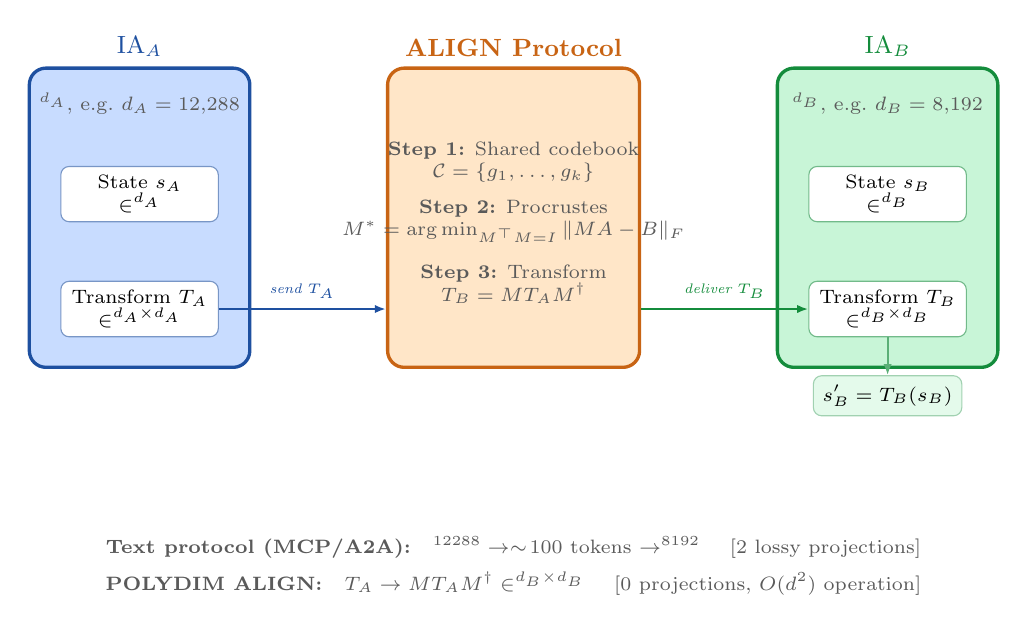
\begin{tikzpicture}[node distance=1.2cm and 2.5cm]

  %% IA_A box
  \node[draw=polyblue, fill=polylightblue, rounded corners=6pt,
        minimum width=2.8cm, minimum height=3.8cm, line width=1.2pt]
    (IA_A) at (0, 0) {};
  \node[above=0pt of IA_A.north, font=\small\bfseries\color{polyblue}]
    {$\mathrm{IA}_A$};
  \node[below=6pt of IA_A.north, font=\scriptsize\color{polygray}]
    {$\RR^{d_A}$, e.g.\ $d_A = 12{,}288$};

  \node[draw=polyblue!60, fill=white, rounded corners=3pt,
        minimum width=2.0cm, font=\scriptsize, align=center]
    (stateA) at (0, 0.3) {State $s_A$\\$\in \RR^{d_A}$};
  \node[draw=polyblue!60, fill=white, rounded corners=3pt,
        minimum width=2.0cm, font=\scriptsize, align=center,
        below=0.2cm of stateA]
    (transA) at (0,-0.6) {Transform $T_A$\\$\in \RR^{d_A \times d_A}$};

  %% IA_B box
  \node[draw=polygreen, fill=polylightgreen, rounded corners=6pt,
        minimum width=2.8cm, minimum height=3.8cm, line width=1.2pt]
    (IA_B) at (9.5, 0) {};
  \node[above=0pt of IA_B.north, font=\small\bfseries\color{polygreen}]
    {$\mathrm{IA}_B$};
  \node[below=6pt of IA_B.north, font=\scriptsize\color{polygray}]
    {$\RR^{d_B}$, e.g.\ $d_B = 8{,}192$};

  \node[draw=polygreen!60, fill=white, rounded corners=3pt,
        minimum width=2.0cm, font=\scriptsize, align=center]
    (stateB) at (9.5, 0.3) {State $s_B$\\$\in \RR^{d_B}$};
  \node[draw=polygreen!60, fill=white, rounded corners=3pt,
        minimum width=2.0cm, font=\scriptsize, align=center,
        below=0.2cm of stateB]
    (transB) at (9.5,-0.6) {Transform $T_B$\\$\in \RR^{d_B \times d_B}$};

  %% ALIGN box in the middle
  \node[draw=polyorange, fill=polylightorange, rounded corners=6pt,
        minimum width=3.2cm, minimum height=3.8cm, line width=1.2pt]
    (align) at (4.75, 0) {};
  \node[above=0pt of align.north, font=\small\bfseries\color{polyorange}]
    {ALIGN Protocol};

  \node[font=\scriptsize, align=center, text=polygray]
    at (4.75, 0.7) {
      \textbf{Step 1:} Shared codebook \\
      $\mathcal{C} = \{g_1, \ldots, g_k\}$
    };
  \node[font=\scriptsize, align=center, text=polygray]
    at (4.75, -0.05) {
      \textbf{Step 2:} Procrustes \\
      $M^* = \arg\min_{M^\top M=I} \|MA-B\|_F$
    };
  \node[font=\scriptsize, align=center, text=polygray]
    at (4.75, -0.85) {
      \textbf{Step 3:} Transform \\
      $T_B = M T_A M^\dagger$
    };

  %% Arrows
  \draw[-{Latex[length=4pt]}, polyblue, line width=0.9pt]
    (transA.east) -- node[above, font=\tiny\itshape] {send $T_A$}
    (align.west |- transA.east);

  \draw[-{Latex[length=4pt]}, polygreen, line width=0.9pt]
    (align.east |- transB.west) --
    node[above, font=\tiny\itshape] {deliver $T_B$}
    (transB.west);

  %% Application
  \node[draw=polygreen!40, fill=polylightgreen!50, rounded corners=3pt,
        font=\scriptsize, align=center, below=0.5cm of stateB]
    (apply) at (9.5,-1.5) {$s_B' = T_B(s_B)$};
  \draw[-{Latex[length=4pt]}, polygreen!70, line width=0.7pt]
    (transB.south) -- (apply.north);

  %% Comparison
  \node[below=2.0cm of align.south, anchor=north,
        font=\scriptsize, align=center, text=polygray] {
    \textbf{Text protocol (MCP/A2A):}\quad
    $\RR^{12288} \to \sim\!100$ tokens $\to \RR^{8192}$
    \quad [2 lossy projections] \\[4pt]
    \textbf{POLYDIM ALIGN:}\quad
    $T_A \to M T_A M^\dagger \in \RR^{d_B \times d_B}$
    \quad [0 projections, $O(d^2)$ operation]
  };

\end{tikzpicture}

\bigskip
%% ============================================================
%% FIGURE 4: Dimensional Type System
%% ============================================================
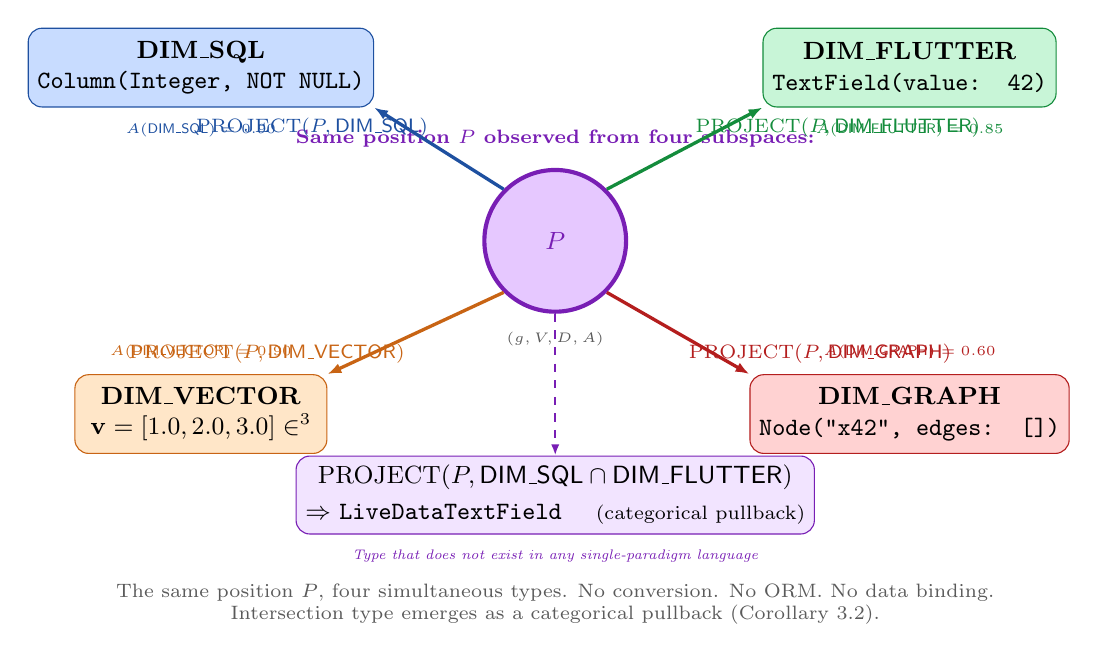
\begin{tikzpicture}[node distance=0.8cm and 1.5cm]

  %% Central position P
  \node[draw=polypurple, fill=polylightpurple, circle,
        minimum size=1.8cm, line width=1.5pt,
        font=\small\bfseries, text=polypurple]
    (P) at (0, 0) {$P$};

  \node[below=3pt of P, font=\tiny\color{polygray}]
    {$(g, V, D, A)$};

  \node[above=4pt of P.north, font=\scriptsize\bfseries, text=polypurple]
    {Same position $P$ observed from four subspaces:};

  %% DIM_SQL projection
  \node[draw=polyblue, fill=polylightblue, rounded corners=5pt,
        minimum width=3.2cm, minimum height=1.0cm,
        font=\small, align=center]
    (sql) at (-4.5, 2.2) {
      \textbf{DIM\_SQL} \\
      \small\texttt{Column(Integer, NOT NULL)}
    };
  \draw[-{Latex[length=5pt]}, polyblue, line width=1.2pt]
    (P.north west) -- node[above left, font=\scriptsize, text=polyblue]
    {$\mathrm{PROJECT}(P, \mathsf{DIM\_SQL})$} (sql.south east);
  \node[below=2pt of sql.south, font=\tiny\itshape, text=polyblue]
    {$A(\mathsf{DIM\_SQL}) = 0.90$};

  %% DIM_FLUTTER projection
  \node[draw=polygreen, fill=polylightgreen, rounded corners=5pt,
        minimum width=3.2cm, minimum height=1.0cm,
        font=\small, align=center]
    (flutter) at (4.5, 2.2) {
      \textbf{DIM\_FLUTTER} \\
      \small\texttt{TextField(value: 42)}
    };
  \draw[-{Latex[length=5pt]}, polygreen, line width=1.2pt]
    (P.north east) -- node[above right, font=\scriptsize, text=polygreen]
    {$\mathrm{PROJECT}(P, \mathsf{DIM\_FLUTTER})$} (flutter.south west);
  \node[below=2pt of flutter.south, font=\tiny\itshape, text=polygreen]
    {$A(\mathsf{DIM\_FLUTTER}) = 0.85$};

  %% DIM_VECTOR projection
  \node[draw=polyorange, fill=polylightorange, rounded corners=5pt,
        minimum width=3.2cm, minimum height=1.0cm,
        font=\small, align=center]
    (vector) at (-4.5, -2.2) {
      \textbf{DIM\_VECTOR} \\
      \small$\mathbf{v} = [1.0, 2.0, 3.0] \in \RR^3$
    };
  \draw[-{Latex[length=5pt]}, polyorange, line width=1.2pt]
    (P.south west) -- node[below left, font=\scriptsize, text=polyorange]
    {$\mathrm{PROJECT}(P, \mathsf{DIM\_VECTOR})$} (vector.north east);
  \node[above=2pt of vector.north, font=\tiny\itshape, text=polyorange]
    {$A(\mathsf{DIM\_VECTOR}) = 0.90$};

  %% DIM_GRAPH projection
  \node[draw=polyred, fill=polylightred, rounded corners=5pt,
        minimum width=3.2cm, minimum height=1.0cm,
        font=\small, align=center]
    (graph) at (4.5, -2.2) {
      \textbf{DIM\_GRAPH} \\
      \small\texttt{Node("x42", edges: [])}
    };
  \draw[-{Latex[length=5pt]}, polyred, line width=1.2pt]
    (P.south east) -- node[below right, font=\scriptsize, text=polyred]
    {$\mathrm{PROJECT}(P, \mathsf{DIM\_GRAPH})$} (graph.north west);
  \node[above=2pt of graph.north, font=\tiny\itshape, text=polyred]
    {$A(\mathsf{DIM\_GRAPH}) = 0.60$};

  %% Intersection type (pullback)
  \node[draw=polypurple, fill=polylightpurple!50, rounded corners=5pt,
        minimum width=4.0cm, minimum height=0.9cm,
        font=\small, align=center, below=1.8cm of P]
    (intersect) {
      $\mathrm{PROJECT}(P, \mathsf{DIM\_SQL} \cap \mathsf{DIM\_FLUTTER})$ \\[2pt]
      \small $\Rightarrow$ \texttt{LiveDataTextField} \quad
      \scriptsize(categorical pullback)
    };
  \draw[-{Latex[length=4pt]}, polypurple, dashed, line width=0.9pt]
    (P.south) -- (intersect.north);
  \node[below=2pt of intersect.south, font=\tiny\itshape, text=polypurple]
    {Type that does not exist in any single-paradigm language};

  %% Caption
  \node[below=0.5cm of intersect.south, anchor=north,
        font=\scriptsize, text=polygray, align=center] {
    The same position $P$, four simultaneous types. No conversion. No ORM. No data binding. \\
    Intersection type emerges as a categorical pullback (Corollary~3.2).
  };

\end{tikzpicture}

\end{document}
